
% Este modelo foi adaptado da versão disponibilizada no site da Engenharia Elétrica da UERJ
% http://www.pel.uerj.br/publico/Modelo_LaTeX_Dissertacao_UERJ.rar
% http://www.pel.uerj.br/defesas/
%
% Utilizei o WinEdt 6.0 com Miktex 2.9
%
% Para gerar o PDF usei a opção PDFTeXfy com o documento [masterthesis.tex] aberto e em foco.
%
% Não consegui usar as figuras em EPS como o modelo original. Usei PNG e JPG sem problemas.
%
%




\documentclass[a4paper,12pt,oneside,openany]{uerj}

\usepackage[english,brazil]{babel}
%\usepackage[latin1]{inputenc}
\usepackage[utf8]{inputenc}
\usepackage{enumerate}
\usepackage{cite}
\usepackage{epsf,epsfig,psfig}
\usepackage{pagina}
\usepackage{indentfirst}
\usepackage{theorem}
\usepackage{fancyhdr}
\usepackage{setspace}
\usepackage{boxedminipage}
\usepackage{float}
\usepackage{makeidx}
\usepackage{amsmath}
\usepackage[hidelinks]{hyperref}




\makeindex


\newtheorem{deff}{Definição}[section]
\numberwithin{equation}{chapter}

\theoremstyle{plain}

\bibliographystyle{plainnat}
\bibliographystyle{unsrt}



\begin{document}

\hypersetup{
    colorlinks,
    citecolor=black,
    filecolor=black,
    linkcolor=black,
    urlcolor=black,
    linktoc=all
}

\thispagestyle{empty}\begin{titlepage}
\begin{center}

	\vspace{-0.5cm}

  \begin{figure}[hbt!]
		\begin{flushleft}
		   
\includegraphics[width=3.44cm,height=3.17cm]{./01_Pre_textuais/logo_uerj_pb.png}
		\end{flushleft}
	\end{figure}
	\vspace{-4cm}

  \hspace{2cm}\large{\textbf{Universidade do Estado do Rio de Janeiro}}\\
  \hspace{2cm}\large{Centro de Tecnologia e Ciências}\\
  \hspace{2cm}\large{Faculdade de Engenharia}\\

  \hspace{2cm}\large{}\\
  \hspace{2cm}\large{}\\
  \hspace{2cm}\large{}\\
  \hspace{2cm}\large{}\\

  \par
  \large{Jéssica Barbosa de Souza}

  \hspace{2cm}\large{}\\
  \hspace{2cm}\large{}\\
  \hspace{2cm}\large{}\\
  \hspace{2cm}\large{}\\


  \par
  \large\textbf{Detecção de falhas em circuitos analógicos utilizando aprendizado de máquinas}


  \par\vfill
  Rio de Janeiro\\2018

\end{center}
\end{titlepage}
\pagebreak\thispagestyle{empty}\begin{center}

Jéssica Barbosa de Souza

% \vfill
\vspace{2cm}

\textbf{Detecção de falhas em circuitos analógicos utilizando aprendizado de máquinas}

\vspace{1.0cm}

\begin{figure}[hbt!]
\begin{center}

\includegraphics[width=10.48cm,height=10.8cm]{./01_Pre_textuais/logo_uerj_gnd_pb.png}
\end{center}
\end{figure}

\vspace{-9cm}
\begin{flushright}
\parbox{8cm}{
\singlespacing{Projeto de graduação apresentado, como requisito parcial para obtenção do grau de Engenheiro Eletricista, à Faculdade de Engenharia, da Universidade do Estado do Rio de Janeiro.}
}
\end{flushright}

\vspace{4.0cm}

Orientador: Prof. Dr. Jorge Luís Machado do Amaral\\

\par\vfill
%\vspace{2cm}

Rio de Janeiro\\2018

\end{center}
\pagebreak\thispagestyle{empty}% Depois de preparar seu trabalho, você deverá enviá-lo para a Biblioteca CTC/B para avaliação do formato e elaboração da Ficha catalográfica.
% Com a ficha pronta (fornecida pela Biblioteca), você poderá alterar este trecho do trabalho em definitivo.
%
% Para este processo, enviei a dissertação em PDF para o email: ctcb.uerj.bdtd@gmail.com (Tratei de todos os detlahes com a Sra. Márcia)
% Qualquer dúvida, veja os contatos da Biblioteca no site da Rede Sirius: http://www.rsirius.uerj.br/
% 


\begin{titlepage}
	\begin{center}
\vfill
\singlespacing
	\vspace*{65mm}
	{CATALOGAÇÃO NA FONTE\\ \vspace{1.5mm}
	UERJ\,/\,REDE SIRIUS\,/\,BIBLIOTECA CTC/B}\\
	\vspace{1.5mm}
	\begin{boxedminipage}{140mm}
	\begin{minipage}{5mm}
		\vspace{-84mm}
		S729
	\end{minipage}
	\hfill
	\raisebox{8.5mm}{
	\begin{minipage}[top]{115mm}
		\vspace*{5mm}

		Souza, Jéssica Barbosa de\\
		\phantom{XX}Detecção de falhas em circuitos analógicos
utilizando aprendizado de máquinas\,/\, Jéssica Barbosa
de Souza. -- 2018.\\
		\phantom{XX}114\,f.\\
		\phantom{XX}\\
		\phantom{XX}Orientadores: Prof. Dr. Jorge Luís Machado do Amaral;\\
\hspace*{5mm}
\
       		\phantom{XX}Projeto Final apresentado à Universidade do Estado
do Rio de Janeiro, Faculdade de Engenharia, para
obtenção do grau de bacharel em Engenharia Elétrica.\\
		\phantom{XX}\\
		\phantom{XX}  1. Aprendizado de maquinas - Monografias. 2.
Detecção de falhas - Monografias. 3. Python -
Monografias. 4. LTspice - Monografias. I. Amaral,
Jorge Luís Machado do. II. Universidade do Estado do
Rio de Janeiro. Faculdade de Engenharia. III. Título.
	\end{minipage}}
	\vspace*{5mm}
	\begin{flushright}
	 CDU~621.3
	\end{flushright}
    \vspace{1mm}
	\end{boxedminipage}\\
	\end{center}
%
	Autorizo, apenas para fins acadêmicos e científicos, a reprodução total ou parcial desta dissertação, desde que citada a fonte.\\
	\noindent
	\begin{tabular}{ccc}
	\phantom{XXXXXXXXXXXXXXXXXXXXXXXXXXXXXX}&	 \phantom{XX}	&	\phantom{XXXXXXXXXXXXXXXX}	\\
	\phantom{XXXXXXXXXXXXXXXXXXXXXXXXXXXXXX}&	 \phantom{XX}	&	\phantom{XXXXXXXXXXXXXXXX}	\\
	\cline{1-1}\cline{3-3}
	Assinatura &		&	Data
	\end{tabular}
\end{titlepage} 
\pagebreak\thispagestyle{empty}\addtocounter{page}{+1}
\begin{center}

Jéssica Barbosa de Souza

\vspace{1cm}

\textbf{Detecção de Falhas em Circuitos Analógicos utilizando métodos de aprendizado de máquinas}

\end{center}

\vspace{.6cm}

\begin{flushright}
\parbox{8cm}{
\singlespacing{Projeto de graduação apresentado, como requisito parcial para obtenção do grau de Engenheiro Eletricista, à Faculdade de Engenharia, da Universidade do Estado do Rio de Janeiro.}
}
\end{flushright}

\vspace{.9cm}


% insira abaixo a data de sua defesa
% Caso não tenha defendido ainda, deixe em branco

\noindent Aprovado em 08 de Outubro de 2018

\noindent Banca Examinadora:


%
%
% Os professores da UERJ DEVEM ser citados primeiro, independente de quem seja o orientador.
%
%



\vspace{1.0cm}

\begin{flushright}
\parbox{13cm}{

\singlespacing

\hrulefill \\

\vspace{-.3cm}
Prof. Dr. Jorge Luís Machado do Amaral (Orientador)
\newline
Faculdade de Engenharia da UERJ
\vspace{1.9cm}

\hrulefill \\

\vspace{-.3cm}
Prof. Dr. Marco Aurélio Botelho da Silva  
\newline
Faculdade de Engenharia da UERJ
\vspace{1.9cm}

\hrulefill \\

\vspace{-.3cm}
Prof. Dr. Douglas Mota Dias
\newline
Faculdade de Engenharia da UERJ
\vspace{.6cm}





}
\end{flushright}
\vfill

\begin{center}
Rio de Janeiro\linebreak 2018
\end{center}

\pagebreak\thispagestyle{empty}\begin{center}
\textbf{DEDICATÓRIA}
\end{center}

$\!$\\

%\vspace{1cm}

\vspace{10cm}
\vfill

\begin{flushright}
    Lute como uma garota!
\linebreak (Autor: Laura Barcella) 
\end{flushright}








\pagebreak\thispagestyle{empty}\begin{center}
\textbf{AGRADECIMENTO}
\end{center}

$\!$\\

Agradeço primeiramente a Deus. Por ter me dado o dom da vida e motivos para continuar buscando meus sonhos. 
Agradeço imensamente aos meus pais, exemplos de dedicação e perseverança diante de todas as adversidades da vida, mesmo sem ter muita instrução, sempre souberam ensinar aos filhos a necessidade de colocar a educação em primeiro lugar. 

Aos meus amigos que me acompanharam desde o inicio da graduação ou ainda nos tempos de colégio militar. Minha eterna gratidão a todas as madrugadas estudando juntos, a amizade nos momentos necessários e desespero em conjunto pelas provas. 

A todos os meus companheiros do Ramo estudantil IEEE UERJ, minha verdadeira segunda casa, onde nos aventuramos nos mais loucos e divertidos desafios. Local onde cresci tanto tecnicamente quanto pessoalmente.  

Ao meu amado namorado, um grande presente que a UERJ me deu, pessoa que me incentiva e alavanca a ir cada vez mais longe. Grande exemplo de dedicação e perseverança, obrigada por estar ao meu lado em todos os momentos e nunca me deixar desistir. Minha eterna gratidão pelo apoio emocional e técnico na elaboração desse projeto. 

E ao meu querido Orientador Jorge amaral, que tanto me ensinou nesses 5 anos de convivência, mostrando a verdadeira função de um grande mestre na vida dos estudantes. Obrigada por toda a paciência e amizade. 


%\pagebreak\thispagestyle{empty}\input{./01_Pre_textuais/Epigrafe}    % não coloquei epígrafe no meu trabalho, mas fica aqui a chamada comentada.
\pagebreak\thispagestyle{empty}\begin{center}
\textbf{RESUMO}
\end{center}

%
% O resumo deve ser organizado em apenas um parágrafo mesmo.
% O número de folha é o número de páginas do PDF -2. Isto ocorre pois na versão final (capa dura) a capa é removida e as duas primeiras páginas são impressas em uma % folha apenas (frente e verso).
%

$\!$\\

\hspace{-1.3cm}\textbf{Souza}, Jéssica B \textit{Detecção de falhas em circuitos analógicos utilizando aprendizado de máquinas}. 114 f. Projeto de Graduação~(Graduação em Engenharia elétrica com ênfase em sistemas eletrônicos) - Faculdade de Engenharia, Universidade do Estado do Rio de Janeiro~(UERJ), Rio de Janeiro, 2018.

\vspace{.2cm}

Este trabalho apresenta uma aplicação real de sistemas inteligentes em projetos de eletrônica. Foram utilizadas técnicas de aprendizado supervisionado para classificar falhas em circuitos analógicos simulados no LTSpice. Entre as duas pontas existe um complexo processo de Extração, Limpeza e pré processamento desses dados. Para isso foram usadas técnicas de \textit{data Cleaning}, \textit{data Mining} e aplicou-se consagrados algoritmos como o PAA (Aproximação Agregada por Partes) e o PCA (Análise das Componentes Principais) para a redução. Ao fim, foram aplicados 10(dez) diferentes algoritmos de aprendizado para a classificação dessas falhas em busca do mais eficiente e robusto para o sistema, sendo todos submetidos a intensos testes também apresentados neste trabalho. Todo o código foi desenvolvido em Python.

\vspace{1cm}

\hspace{-1.3cm}Palavras-chave: Aprendizado de máquina, LTspice, Classificação, Python.
\pagebreak\thispagestyle{empty}\begin{center}
\textbf{ABSTRACT}
\end{center}

$\!$\\

% O resumo em inglês deve ser organizado em apenas um parágrafo mesmo.


\hspace {-1.3cm} \textbf {Souza}, Jessica B \textit{Detection of faults in analog circuits using machine learning}. 114 f. Graduation Project ~ (Graduation in Electrical Engineering with emphasis on electronic systems)  - Faculdade de Engenharia, Universidade do Estado do Rio de Janeiro~(UERJ), Rio de Janeiro, 2018.

This paper presents a real application of intelligent systems in electronics projects. Supervised learning techniques were used to classify faults in simulated analog circuits in LTSpice. Between the two ends there is a complex process of Extraction, Cleaning and pre-processing of this data. For this purpose, data cleaning techniques were used, data mining was used, and algorithms such as the PAA (Approximation Aggregated by Parts) and PCA (Major Component Analysis) were applied for the reduction. Finally, ten (10) different learning algorithms were applied to the classification of these faults in search of the most efficient and robust for the system, all of which were submitted to intense tests also presented in this work. All code was developed in Python.

\vspace{1cm}

\hspace{-1.3cm}Keywords: Machine-Learning, classification , LTSpice, Python.

\fancypagestyle{plain}{
\fancyhf{} % clear all header and footer fields
\renewcommand{\headrulewidth}{0pt}
\renewcommand{\footrulewidth}{0pt}}
\pagestyle{plain}

\pagebreak

\def\listfigurename{LISTA DE FIGURAS}\listoffigures

\def\listtablename{LISTA DE TABELAS}\listoftables


\newpage

\begin{center}
\textbf{LISTA DE SIGLAS}
\end{center}
$\!$\\

\begin{tabular}{lll}


APCA & \hspace{1cm} &  Adaptive Piecewise Constant Approximation \\
ctsv  & \hspace{1cm} & continuous-time state-variable \\
PAA  & \hspace{1cm} &  Piecewise Aggregate Approximation \\
SK  & \hspace{1cm} &  Sallen-Key \\
SVDD  & \hspace{1cm} & support vector data description \\
DFT & \hspace{1cm} & Traformada Discreta de Fourier\\
DWT & \hspace{1cm} &Transformada Discreta Wavelet \\
POD & \hspace{1cm} & transformada de Hotelling ou decomposição ortogonal própria \\
CC & \hspace{1cm} & Corrente Continua\\
V & \hspace{1cm} & Volts\\
ETL & \hspace{1cm} & Extração, Transformação e Limpeza\\
SGD & \hspace{1cm} & Descentramento Estocástico de Gradiente\\
PCA & \hspace{1cm} & Análise dos principais componentes\\
\end{tabular}
    % não coloquei LISTA DE SIGLAS no meu trabalho, mas fica aqui a chamada comentada.
\def\contentsname{SUMÁRIO}\tableofcontents

\fancypagestyle{plain}{
\fancyhf{} % clear all header and footer fields
\fancyhead[R]{\thepage}
\setlength{\voffset}{-1cm}
\setlength{\headsep}{1cm}
\renewcommand{\headrulewidth}{0pt}
\renewcommand{\footrulewidth}{0pt}}

\pagestyle{plain}

\pagebreak
\addcontentsline{toc}{chapter}{\hspace{1.7cm}\bfseries INTRODUÇÃO}
\noindent\textbf{INTRODUÇÃO}
$\!$\\


A otimização de tarefas manuais é uma necessidade em diversos campos de pesquisa, e nesse sentido o desenvolvimento de estratégias de teste visando detectar e diagnosticar falhas em circuitos analógicos ou digitais tem se mostrado uma tarefa desafiadora e encorajadora, de uma boa quantidade de pesquisas, devido ao grande número de aplicações que demandam testes e ao alto custo dos mesmos. Muitas áreas, tais como telecomunicações, multimídia e aplicações biomédicas, precisam de bom desempenho em aplicações de alta frequência, baixo ruído e baixa potência, o que somente pode ser alcançado usando circuitos integrados analógicos e de sinais mistos. Assim, automatizar os processos de detecção e diagnóstico de falhas nesses circuitos é muito importante\cite{ALBUSTANI}.

Com a evolução dos processos de eletrônica, circuitos foram cada vez mais encapsulados: o que antes continha um componente, agora contém um circuito inteiro. Neste nível de integração, esse tipo de circuito gera problemas difíceis de teste e projeto. As causas são a falta de bons modelos de falhas, falta de um padrão de projeto com vistas à testabilidade e o aumento da importância das falhas relacionadas ao tempo . Portanto, a estratégia de testes para detecção e diagnóstico de falhas ainda é severamente dependente da perícia e da experiência que os engenheiros têm sobre as características do circuito. Assim, a detecção e a identificação de falhas é  um processo interativo e que consome bastante tempo \cite{amaral}. 

Nas últimas décadas, uma boa quantidade de pesquisas em diagnósticos de falhas foi concentrada em desenvolver ferramentas que facilitassem as tarefas de diagnóstico. Embora tenha havido progressos importantes, essas novas tecnologias não tem sido largamente aceitas. Isso motiva os pesquisadores a desenvolver novas estratégias para o diagnóstico.  

Estratégias envolvendo classificadores procuram por comportamentos específicos de falhas e tornam-se vulneráveis quando existe superposição dos padrões de falha ou quando têm que tratar padrões de falha que não foram apresentados a eles durante a fase de treinamento. Considerando que no conjunto de falhas apresentado não há superposição, esse método se torna eficaz e assertivo.

Este trabalho apresenta o desenvolvimento de um sistema de detecção de falhas para circuitos lineares e invariantes no tempo, onde o comportamento do circuito é representado pela Aproximação Agregada por Partes (PAA - Piecewise Aggregate Approximation) da resposta ao impulso do circuito. Os experimentos são realizados nos circuitos "Filtro Passa-Banda Sallen Key", "Filtro Universal", "Retificador Não-Linear" e "CTSV" (Continuous-Time State-Variable). Para cada um dos circuitos foram executados diferentes algoritmos de predição a fim de determinar qual algoritmo atinge a melhor precisão.

Este trabalho é dividido da seguinte forma: o capítulo 1 apresenta a justificativa e objetivos; o capítulo 2 aborda a detecção de falhas e seus os conceitos básicos; o capítulo 3 apresenta os algoritmos utilizados e seu conceito; o capítulo 4 descreve o estudo de caso para cada um dos circuitos.  



\chapter{Justificativa e Objetivo}
\label{chapter:exemplo}

\section{\textbf{Justificativa}}
\label{sec:CapJustificativa}

As técnicas de aprendizado de máquinas, apesar de terem uma infinita gama de aplicações, muitas vezes não são bem compreendidas e aplicada. Quando as relacionamos com conceitos de engenharia, por exemplo, que saem puramente da computação, essas técnicas são mistificadas. 

Com a vontade de unir três grandes áreas de interesse do autor ( Programação, eletrônica e análise de dados) surgiu o interesse em dar prosseguimento a este trabalho, demonstrando o poder que a união entre teoria e pratica podem ter. 

Uma outra motivação é incentivar o estudo mais aprofundado de técnicas de algoritmos mais avançadas. Agregando ainda mais na formação como engenheira. 

\section{\textbf{Objetivo}}
\label{sec:CapObjetivo}

Este projeto objetiva unir conceitos de Engenharia Elétrica com Ciência de Dados para resolver problemas reais.

Através da implementação de técnicas de aprendizado de máquina serão elucidados métodos para a  previsão da existência de falhas em circuitos ou confirmação do perfeito funcionamento. 

A primeira etapa deste métodos, consiste na aquisição de dados sobre o circuito a ser analisado. A obtenção destes dados será obtida a partir da simulação do circuito. Posteriormente, serão aplicadas análise, limpeza e redução destes dados. 

Por fim, o objetivo deste projeto é mostrar a aplicação prática de técnicas de \textit{Machine Learning} na predição eficaz de falhas em circuitos. Esse fluxo é descrito na \ref{fig:diagrama}. 


\begin{figure}[H]
\begin{center}
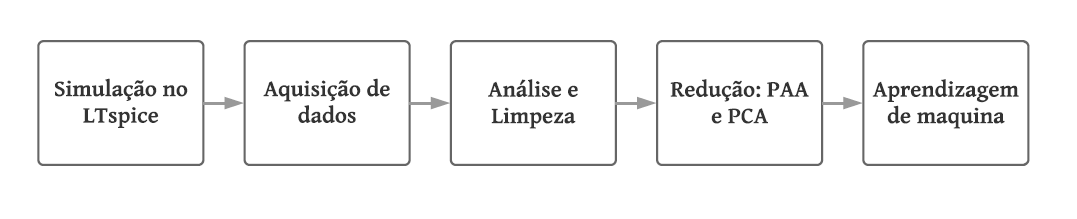
\includegraphics[width=13cm]{./02_Cap1/figures/diagrama.PNG}
\caption{\label{fig:diagrama}- Diagrama do fluxo de informação dos dados}
\end{center}
\end{figure}




\chapter{Detecção de Falhas em circuitos}

O diagnóstico de falhas é um grande desafio frente à crescente complexidade dos circuitos analógicos e de sinais mistos. Em primeiro lugar, os circuitos analógicos não possuem um padrão de saída pré-determinado como em circuitos digitais (Alto ou baixo), havendo para cada circuito características próprias de sinais, operações e restrições. Isto explica o pequeno número de modelos de falhas para estes tipos de circuitos, ao contrário que ocorre nos circuitos digitais. O segundo ponto é que, dependendo do tipo de detecção realizado, há dificuldade de se acessar o atributo desejado sem alterar as características do circuito. Por exemplo, existe uma dificuldade de medir correntes sem alterar as conexões originais do circuito \cite{BANDLER}. Outra razão para esta dificuldade está no fato de que um circuito analógico tem seus parâmetros definidos a partir dos componentes nele utilizados. Dessa forma, o número de combinações de falhas, ou de comportamentos normais, pode ser muito grande, o que torna o uso de métodos determinísticos pouco eficazes.


Os métodos conhecidos em geral esbarram em dificuldades similares como grande volume de dados, dificuldade computacional e  variedade de falhas mesmo considerando o grande avanço tecnológico da computação\cite{DUHAMEL}.

Nas últimas décadas, a pesquisa na área de diagnóstico de falhas concentrou-se em desenvolver ferramentas que simplifiquem o processo de diagnóstico \cite{FENTON}. As principais ferramentas utilizadas têm sido métodos de inteligência computacional para o diagnóstico. Mesmo tendo ocorrido progressos significativos, estas novas tecnologias ainda não são amplamente aceitas. Tais técnicas são normalmente baseadas na utilização de classificadores para a distinção entre as falhas, ao extrair atributos dos sinais de tensão e corrente do circuito quando submetido à alguma condição específica. Na sequência, submete-se o classificador a um treinamento e, avalia-se o desempenho da classificação na detecção das falhas no circuito. Entretanto, esta abordagem exige que as classes de falha sejam cuidadosamente escolhidas. Além disso, este tipo de classificador só é capaz de indicar classes de falha para as quais ele tenha sido treinado, caso contrário é necessário que se efetue o treinamento da classe desconhecida antes da análise para não haver a classificação incorreta da falha.

\section{\textbf{Conceito Básico}}

O termo falha é citado em trabalhos de diversas áreas. Em \cite{WEBER} é chamada de falha a causa física de um erro, a alteração que gera o defeito, que é o estado de desvio de um componente ou sistema, no caso da computação.
Para o caso deste trabalho, definimos falha como o comportamento anormal ou o defeito em um componente, sistema ou dispositivo que pode levar a um mau funcionamento. Ou seja, a falha é a diminuição parcial ou total da capacidade de um sistema de desempenhar a função para o qual é projetado, por um certo período de tempo ou permanentemente \cite{lombardi}.

\section{\textbf{Tipos de Falhas}}

Os tipos de falhas que um circuito pode apresentar são bastante abrangentes. As falhas podem ser determinadas pelo seu tipo de desvio, por sua duração, pela quantidade de dispositivos a apresentar falha ao mesmo tempo, à sua observabilidade e à sua distinção.

Quanto ao grau de desvio, uma falha é dita paramétrica quando a sua ocorrência está relacionada a um desvio do parâmetro no tempo, não alterando a topologia do circuito. Quando a falha possui um desvio extremo de parâmetro, ela é então chamada de falha catastrófica. Isto porque este tipo de falha está relacionado à perda de componentes do sistema, alterando a sua estrutura topológica, assim como a sua própria função de transferência \cite{LUO}. Por exemplo, em circuitos elétricos, circuito aberto e curto-circuito são falhas catastróficas \cite{DUHAMEL}.

Quanto ao número de falhas simultâneas que ocorrem em um circuito, a falha é dita simples quando sua ocorrência é única, havendo a mudança paramétrica de um único componente. Por outro lado, a falha é dita múltipla quando, em sua ocorrência, há a mudança paramétrica de mais de um componente simultaneamente. Quanto à relação entre falhas, duas ou mais falhas são independentes se não existem relações de causa e efeito entre suas ocorrências, caso contrário, elas são dependentes \cite{lombardi}.

Com relação à sua duração, uma falha é dita intermitente quando a sua ocorrência existe por um certo período de tempo aleatório e imprevisível, alternando-se entre o comportamento normal e anormal. Por outro lado, quando a ocorrência da falha é contínua ao longo do tempo, sendo o reparo do componente defeituoso a única solução para a sua interrupção, a falha é dita permanente. O termo transiente é também usado por alguns autores para classificar falhas causadas por mudanças temporárias no ambiente onde o circuito está operando. Por sua vez, o termo incipiente é utilizado para nomear falhas que evoluem gradualmente, tornando-se mais severas ao longo do tempo \cite{MANDERS}.

Por fim, quanto à sua observabilidade, duas ou mais falhas são classificadas como mascaráveis quando suas ocorrências simultâneas ou progressivas podem compensar seus efeitos, tornando o sistema livre de erros sob certas condições \cite{lombardi}. Quando uma falha apresenta um efeito sobressalente à sua ocorrência no circuito, isolada ou simultânea, ela é chamada de falha dominante. As falhas são chamadas de indistintas quando os seus efeitos afetam o circuito de modo que seus efeitos sejam distinguíveis entre si.

Por fim, as falhas inconfundíveis são aquelas cujo efeitos são atribuídos a uma única e determinada condição, podendo ser reveláveis em certas condições (detectáveis), ou não-detectáveis, caso contrário.

Todos essas variações apresentadas fazem o diagnostico ser algo complexo e relevante para as pesquisas. 





%\chapter{Ferramentas do Projeto}

\chapter{ALGORITMOS DE APRENDIZADO DE MÁQUINAS}

As técnicas de aprendizagem de máquinas surgiram da necessidade de otimização de detecção de padrões não explícitos. Dentre as diferentes aplicações no mercado de trabalho, existe a detecção de fraudes, analise de currículo e Previsão de falha de equipamentos, por exemplo em 
\cite{santander}.

Oito algoritmos foram escolhidos para realização dos testes. Cada um desses algoritmos é descrito neste capítulo, com suas principais vantagens e desvantagens.

\section{\textbf{Supervisionada}}
Na aprendizagem supervisionada treinamos os algoritmos utilizados, dados que já temos o gabarito, ou seja, já foram mapeados com as saídas desejadas. O algoritmos deverá ter a capacidade de se treinar e comparar o resultado previsto com o idealizado. 

Problemas de aprendizagem supervisionada são classificados em problemas de “regressão” e “classificação”. Em um problema de regressão, objetiva-se prever os resultados em uma saída contínua, o que significa que é desejado mapear variáveis de entrada para alguma função contínua. Em um problema de classificação, objetiva-se prever os resultados em uma saída discreta, isto é, o objetivo é mapear variáveis de entrada em categorias distintas\cite{aprendizagem}.

Exemplo:
 \renewcommand{\theenumi}{\Alph{enumi}}
 \begin{enumerate}
 
    \item Regressão - Dada uma imagem de homem/mulher, temos de prever sua idade com base em dados da imagem.
    \item Classificação - Dada um exemplo de tumor cancerígeno, temos de prever se ele é benigno ou maligno através do seu tamanho e idade do paciente.
     
 \end{enumerate}


Foram usado diferentes algoritmos para determinar aquele com melhor eficácia para o sistema. 
\subsection{{Classificador por Árvore de decisão}}

A árvore de classificação é o resultado de se fazer uma sequência ordenada de perguntas, e as perguntas feitas a cada passo na sequência dependem das respostas às perguntas anteriores. A sequência termina em uma previsão da classe.
O ponto de partida de uma árvore de classificação é chamado de nó raiz e consiste em todo o conjunto de aprendizado, e está no topo da árvore. Um nó é um subconjunto do conjunto de atributos, e pode ser terminal ou não-terminal. Um nó não-terminal é um nó que se divide em nós filhos. Tal divisão é determinada por uma condição sobre o valor de um único atributo, e que vai dividir os exemplos de acordo com a condição, em outros nós. Um nó que não se divide é chamado de nó terminal, e a ele é atribuída uma classe. Cada exemplo no conjunto cai em um dos nós terminais. 

Uma árvore de decisão é um mapa dos possíveis resultados de uma série de escolhas relacionadas. Geralmente começa com um único nó, que se divide em possíveis resultados. Cada um desses resultados leva a nós adicionais, que se ramificam em outras possibilidades. Assim, cria-se uma forma de árvore. Tem alta taxa de compreensão dos dados, mas podem se tornar excessivamente complexas e por consequência pesadas. A \ref{fig:arvoredecisao} mostra de forma simplificada como é feita essa categorização. 


\begin{figure}[H]
\begin{center}
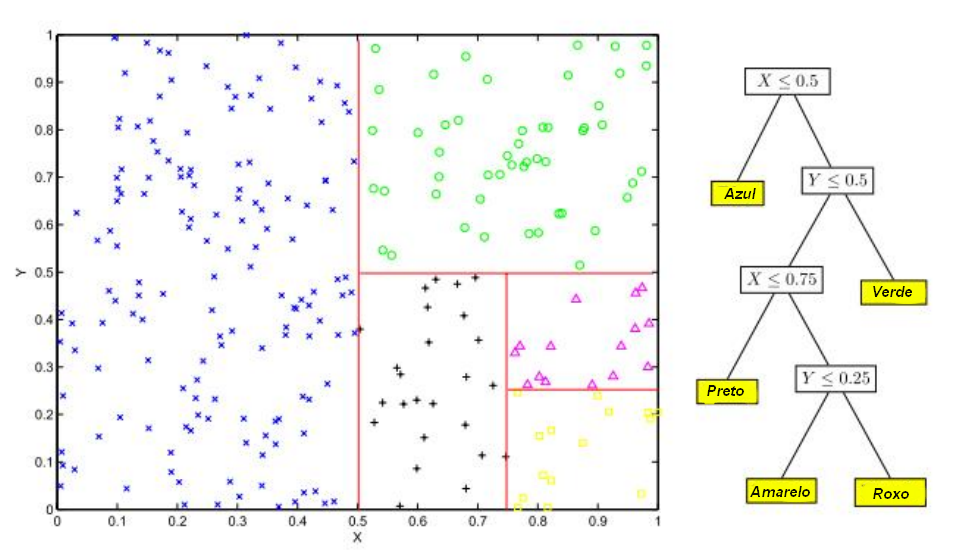
\includegraphics[width=13cm]{./02_Cap2/figures/arvore_de_decisao.png}
\caption{\label{fig:arvoredecisao}- Exemplo de partições em árvores de decisão.}
\end{center}
\end{figure}

O processo de crescimento de uma árvore de classificação necessita responder a quatro questões básicas: Como escolher as condições para dividir cada nó? Que critério devemos usar para dividir um nó pai em seus nós filhos? Como vamos decidir quando um nó se tornará um nó terminal (parar a divisão)? Como vamos atribuir uma classe a esse nó terminal?

Existe uma série de equações que ajudam o algorítimo a responder às perguntas levantadas. A principal delas é a de entropia que caracteriza a impureza dos dados, num conjunto, ela caracteriza a falta de homogeneidade dos dados de entrada em relação à sua classificação. Por exemplo, a entropia é máxima (igual a 1) quando o conjunto de dados é heterogêneo e miníma (igual a 0) quando os dados são totalmente homogêneos. Dado um conjunto de entrada S que pode ter c classes distintas e tendo pi o identificador de quantos de dados em S que pertence a classe i. a entropia de S será dada por:
\begin{equation}
E(S) = \sum_{i=1}^{c}-pi*log(pi)
\end{equation}
Utilizando essa equação, o código consegue saber se os dados estão homogêneos e se deve ou não criar novos nós de decisão\cite{arvored}. 




\subsection{{Classificador AdaBoost}}

O AdaBoost é um algoritmo de aprendizado supervisionado do tipo boost. Seu nome deriva de Adaptive Boosting, no sentido que ele é adaptado através de um sistema de pesos durante sua execução.O AdaBoost combina um conjunto de funções simples de classificação, denominadas classificadores fracos (como a arvore de decisão) para formar um classificador forte. 
Um classificador forte é composto de um conjunto de classificadores fracos, associados
a pesos que classificam de forma precisa dois conjuntos de dados pré-rotulados, onde as
características com pesos maiores são mais significativas para a classificação de exemplos definidos como parte de um certo conjunto. Na Equação a seguir é formalizada a criação de um classificador forte através de um algoritmo de Boosting.
\begin{equation}
H(x) = α1h1 + α2h2 + ... + αnhn(x)
\end{equation}
onde \[H(x)\] é um classificador forte, αi é o peso associado ao classificador hi. 
Dado uma base de dados de entrada, a função do AdaBoost é encontrar o conjunto de características que comporão o classificador forte provendo uma melhor classificação do conjunto de entrada\cite{AdaBoost}.




\subsection{{Classificador Floresta aleatória}}

Floresta Aleatória (Random Forest) é um algoritmo de aprendizagem de máquina flexível que produz excelentes resultados a maioria das vezes, mesmo sem ajuste de hiperparâmetros. É também um dos algoritmos mais utilizados, devido à sua simplicidade e o fato de que pode ser utilizado para tarefas de classificação e também de regressão. 

O algoritmo cria uma floresta de um modo aleatório. A “floresta” criada é uma combinação de árvores de decisão como demostra a \ref{fig:randomfloresta}, na maioria dos casos treinados com o método de bagging ( estimador aleatório). A idéia principal do método de bagging é que a combinação dos modelos de aprendizado aumenta o resultado geral.


\begin{figure}[H]
\begin{center}
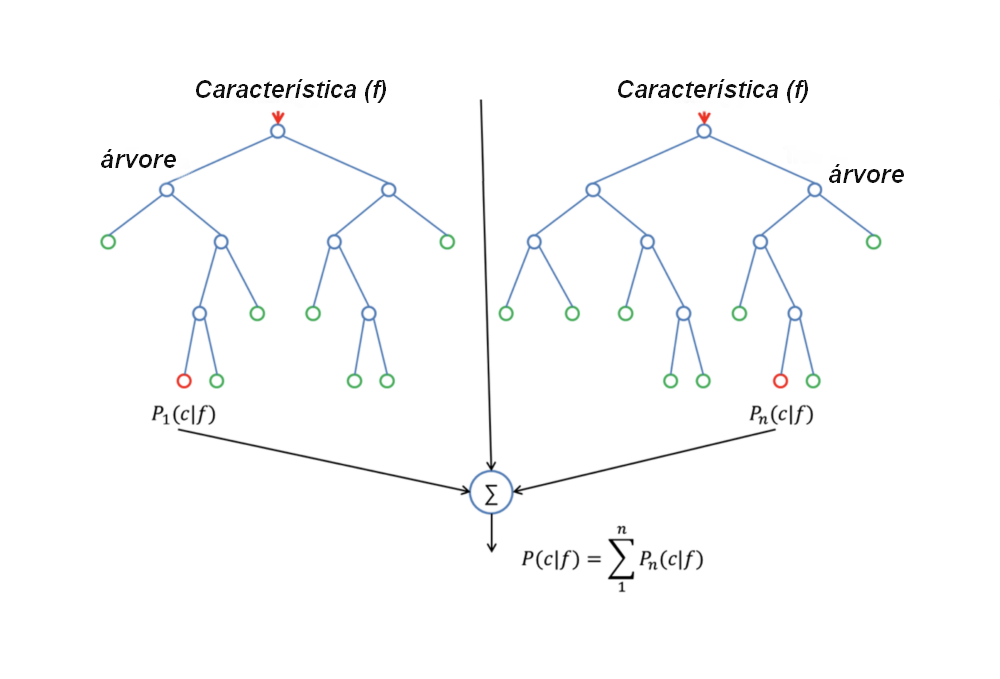
\includegraphics[width=13cm]{./02_Cap2/figures/forestRandom.png}
\caption{\label{fig:randomfloresta}- Floresta aleatória.}
\end{center}
\end{figure}



 A floresta aleatória adiciona aleatoriedade extra ao modelo, quando está criando as árvores. Ao invés de procurar pela melhor característica ao fazer a partição, ele busca a melhor característica em um subconjunto aleatório das características. Este processo cria uma grande diversidade, o que geralmente leva a geração de modelos melhores.

Uma grande vantagem do algoritmo de florestas aleatórias é que ele pode ser utilizado tanto para tarefas de classificação quanto para regressão, o que representa a maioria dos sistemas de aprendizagem de máquina atuais.

Outra grande qualidade das florestas aleatórias é a facilidade para se medir a importância relativa de cada característica para a predição. É possível medir  a relevância das características analisando quantos nodos das árvores, que usam uma dada característica, reduzem impureza geral da floresta, ou seja, aumenta a precisão da decisão não deixando a predição ser alterada por ruídos. Ele calcula este valor automaticamente para cada característica após o treinamento e normaliza os resultados para que a soma de todas as importâncias seja igual a 1. Isso ajuda a escolher quais variáveis utilizadas estão realmente influenciando nos dados finais\cite{Floresta}. 


\subsection{{Classificador Gaussiano de Naive Bayes}}

O algoritmo Naive Bayes é um classificador probabilístico baseado no “Teorema de Bayes”, o qual foi criado por Thomas Bayes (1701 - 1761) para tentar provar a existência de Deus.
Tornou-se popular na área de Aprendizado de Máquina para categorizar textos baseado na frequência das palavras usadas, e assim pode ser usado para identificar se determinado e-mail é um SPAM ou sobre qual assunto se refere determinado texto, por exemplo.

É matematicamente muito simples e rápido comparado a outros classificadores. Além disso, o Naive Bayes só precisa de um pequeno número de dados de teste para concluir classificações com uma boa precisão\cite{Bayes}.

 Sua característica marcante é ele desconsiderar completamente a correlação entre as variáveis. Dessa Forma cada variável é tratado, cada um, de forma independente entre si.  

O algoritmo de Naive Bayes consiste em encontrar a probabilidade Futura multiplicando a probabilidade inicial dado a probabilidade condicional, conforme a equação a seguir \cite{Bayes2}. 
\begin{equation}
P(A\mid B )= \frac{P(B\mid A )*P(A)}{P(A)}
\end{equation}


\subsection{{Classificador K vizinhos mais próximos}}

A ideia principal do KNN é determinar o rótulo de classificação de uma amostra baseado nas amostras vizinhas advindas de um conjunto de treinamento. Na \ref{fig:knn} é exemplificada uma aplicação, na qual temos um problema de classificação com dois rótulos de classe e com k = 7. No exemplo, são aferidas as distâncias de uma nova amostra, representada por uma estrela, às demais amostras de treinamento, representadas pelos circulos azuis e amarelas. A variável k representa a quantidade de vizinhos mais próximos que serão utilizados para averiguar a qual classe a nova amostra pertence. Com isso, das sete amostras de treinamento mais próximas da nova amostra, 4 são do rótulo A e 3 do rótulo B. Portanto, como existem mais vizinhos do rótulo A, a nova amostra receberá o mesmo rótulo deles, ou seja, A.

\begin{figure}[H]
\begin{center}
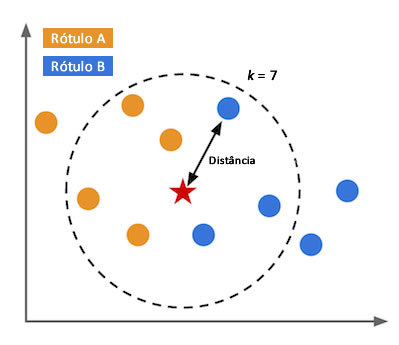
\includegraphics[width=7cm]{./02_Cap2/figures/imgKnn.png}
\caption{\label{fig:knn}- classificação do KNN com dois rótulos de classe e k = 7.}
\end{center}
\end{figure}

Dois pontos chaves que devem ser determinados para aplicação do KNN são: a métrica de distância e o valor de k. Para métrica de distância a mais utilizada é a distância Euclidiana, descrita na equação a seguir.
\begin{equation}
 D = \sqrt{(p_1 - q_1)^2 + \cdots + (p_n - q_n)^2} = \sqrt{\sum_{i=1}^n (p_i - q_i)^2}
 \end{equation}

onde $$P = (p_1, \cdots, p_n)$$  e $$Q = (q_1, \cdots, q_n)$$ são dois pontos n -dimensionais. 

A grande vantagem do KNN é sua abordagem simples de ser compreendida e implementada. Todavia, calcular distância é tarefa custosa e caso o problema possua grande número de amostras o algoritmo pode consumir muito tempo computacional. Além disso, o método é sensível à escolha do k que não possui um valor estabelecido, será variável com os dados\cite{knn}. 



\subsection{{Classificador Gradiente de descida estocástica}}

A Descida do Gradiente é uma ferramenta padrão para otimizar funções complexas iterativamente dentro de um programa de computador. Seu objetivo é encontrar um mínimo. Para as funções mais complexas pode haver muitos mínimos, a função de uma otimização seria encontrar o melhor mínimo. 

A Descida do Gradiente pode ser lenta para executar em conjuntos de dados muito grandes. Como uma iteração do algoritmo de descida do gradiente requer uma previsão para cada instância no conjunto de dados de treinamento, pode demorar muito quando existe milhares de instâncias.

Em situações em que se possui grandes quantidades de dados, você pode usar uma variação da descida do gradiente chamada Gradiente de descida estocástica.

Nesta variação, o procedimento de descida do gradiente é executado, mas a atualização para os coeficientes é realizada para cada instância de treinamento, em vez do final do lote de instâncias.

O primeiro passo do procedimento exige que a ordem do conjunto de dados de treinamento seja aleatória. Isto é, misturar a ordem que as atualizações são feitas para os coeficientes. Como os coeficientes são atualizados após cada instância de treinamento, as atualizações serão intensas, e assim o custo correspondente funcionará. Ao misturar a ordem para as atualizações dos coeficientes, ela aproveita essa caminhada aleatória e evita que ela fique “distraída” ou presa.

O procedimento de atualização para os coeficientes é o mesmo que o anterior, exceto que o custo não é somado em todos os padrões de treinamento, mas sim calculado para um padrão de treinamento.

A aprendizagem pode ser muito mais rápida com descida de gradiente estocástica para conjuntos de dados de treinamento muito grandes e muitas vezes apenas se precisa de um pequeno número de passagens através do conjunto de dados para alcançar um conjunto de coeficientes bom o suficiente \cite{gradiente}.



\subsection{{Classificador de Regressão logística}}

A regressão logística pode ser definida como um tipo de análise de regressão
muito semelhante a regressão linear. A diferença sutil entre os dois modelos é que
enquanto na regressão linear temos um valor real como saída, na regressão logística
temos um resultado binário. Ou seja, a partir de um determinado valor a saída torna-se “0” e no contrário temos um valor “1”. Dentre diversas aplicações, a mais direta é para o uso de classificação. 

É útil para modelar a probabilidade de um evento ocorrer como função de outros fatores.
 regressão logística analisa dados distribuídos binominalmente da forma:
 
\begin{equation}
     Y_{i}\ \sim B(p_{i},n_{i}),{\text{ for }}i=1,\dots ,m,
\end{equation}
Onde os números de ensaios de Bernoulli ni são conhecidos e as probabilidades de êxito pi são desconhecidas. O modelo é então obtido na base de que cada ensaio (valor de i) e o conjunto de variáveis explicativas/independentes possa informar acerca da probabilidade final \cite{logistica}.

\subsection{{Classificador Máquinas de vetores de suporte}}

Os fundamentos de SVM são provenientes da Teoria de Aprendizagem Estatística desenvolvida
inicialmente pelo pesquisador russo Vladmir Vapnik e colaboradores \cite{Vanpick} que idealizaram o princípio indutivo de Minimização do Risco Estrutural.

Embora as pesquisas desenvolvidas com SVM sejam recentes, as raízes do método foram
formuladas na década de 70. Inicialmente o método tinha dois problemas que foram resolvidos na década de 90 que iniciaram uma era de pesquisas com esse método.  
Essa aplicação categoriza as classes reconhecendo suas diferenças, assim podemos obter um padrão complexo dos dados mesmo sem ter um conhecimento prévio acerca do comportamento. Dessa forma, ele funciona de maneira similar a uma caixa preta, recebendo entradas e gerando uma saída que pode ser muito útil para encontrar padrões em dados que são muito complexos e não óbvios.

Uma das melhores características das máquinas de vetores de suporte é que elas são capazes de lidar muito bem com erros e ruídos nos dados. Elas são geralmente capazes de perceber o padrão de fundo nos dados e filtrar valores de dados atípicos e outras complexidades \cite{MetaQuotes}.








\chapter{MODELO PROPOSTO}

Foi proposta a execução do projeto em seis partes descritas a seguir. 

\section{\textbf{Simulação dos circuitos}}

O LTspice é um software de simulação que pode ser utilizado para simular e analisar o comportamento e funcionamento de um circuito elétrico, contendo uma grande variedade de componentes  como, por exemplo, transistores, diodos, resistores e capacitores \cite{Spice}.

Esta ferramenta possibilita que o usuário estime com bastante precisão, através de vários tipos de simulações, o comportamento de circuitos elétricos dos mais variados tamanhos e níveis de complexidade.
Para que o SPICE possa realizar tais estimativas, via simulação, o usuário deve fornecer ao software os seguintes dados\cite{LTSpice}:
\renewcommand{\theenumi}{\Alph{enumi}}
 \begin{enumerate}
\item  Descrição do circuito: Elementos, fontes de sinais e de polarização, e principalmente como estes dispositivos estão interligados no circuito. É necessário o fornecimento dos parâmetros modelares para a descrição comportamental dos componentes ativos a serem simulados.

\item  Especificação de análise: Tipos de análise a serem executadas (CC, transiente, pequenos sinais etc.)

\item  Especificação dos resultados: Tipo de resultado esperado da simulação, como correntes e tensões específicas.
\end{enumerate}

Um dos grandes diferenciais do LTspice é a possibilidade de programar o comportamento dos componentes no decorrer da simulação. Assim é possível, através de configurações de parâmetros, induzir comportamentos imprevistos, simular a resposta para condições extremas ou fornecer diferentes tipos de entrada dentre outras alterações. 

Devido às características apresentadas, este  foi o simulador escolhido para o projeto. Foram usadas quatro topologias conhecidas para a obtenção dos dados, dentro das quais foram escolhidos, aleatoriamente, componentes cujos valores sofreram variações durante a simulação (ora com valores altos, ora com valores extremamente baixos). Estas alterações objetivam provocar falhas que influenciam na tensão de saída do sistema, sendo cada falha provocada de forma única e isolada. 


\begin{enumerate}
    \item[Circuito I - ] \textbf{\textit{Sallen Key:}} Este é um circuito passa-banda ativo de 2ª Ordem, projetado neste trabalho com 1 amplificador operacional como o núcleo do circuito, 5 resistores e 2 capacitores, a qual é a configuração mais básica deste tipo de arquitetura. A sua arquitetura é mostrada na \ref{fig:Circuito1}. Este é o principal circuito utilizado no estudo de detecção de falhas, devido à sua baixa sensibilidade aos parâmetros passivos do circuito \cite{Cbrn2009}. 


\begin{figure}[H]
\begin{center}
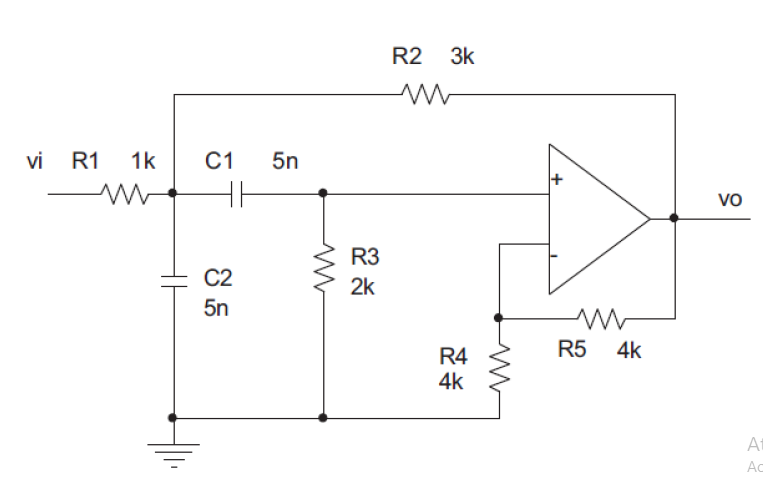
\includegraphics[width=12cm]{./04_Cap4/figures/sallenckt.png}
\caption{\label{fig:Circuito1}- Circuito :{\textit{ Sallen Key}}}
\end{center}
\end{figure}

 
Para simular falhas neste circuito são realizadas alterações nos valores dos resistores R1, R2 e R3  e dos capacitores C1 e C2. Essa variação esta visível na \ref{tab:falhasckt1}.

 \begin{table}[H]
         \centering
        \begin{tabular}{ccc}
        \textbf{Grupo} & \textbf{Simulação} & \textbf{Classificação do Erro} \\
   1              & 0-299              & R1 Alto                        \\
        2              & 300-599            & R1 Baixo                       \\
        3              & 600-899            & R2 Alto                        \\
        4              & 900-1199           & R2 Baixo                       \\
        5              & 1200-1499          & R3 Alto                        \\
        6              & 1500-1799          & R3 Baixo                       \\
        7              & 1800-2099          & C1 Aberto                      \\
        8              & 2100-2399          & C1 Curto                       \\
        9              & 2400-2699          & C2 Aberto                      \\
        10             & 2700-2999          & C2 Curto                       \\
        11             & 3000-3299          & Normal                     \end{tabular}
        \caption{\label{tab:falhasckt1}- Falhas circuito 1}
\end{table}  


    

 \item[Circuito II - ]    \textbf{\textit{Biquad Highpass Filter}}: O Filtro Passa Alta Ativo de segunda ordem é obtido com 4 amplificadores operacionais na parte ativa do circuito, 10 resistores e 2 capacitores, totalizando 12 componentes passivos e 16 componentes no total. A sua arquitetura é mostrada na \ref{fig:Circuito2}. Este circuito também é bastante utilizado no estudo de detecção de falhas por sua baixa sensibilidade à variação dos parâmetros passivos \cite{lombardi} . 
 

    
\begin{figure}[H]
\begin{center}
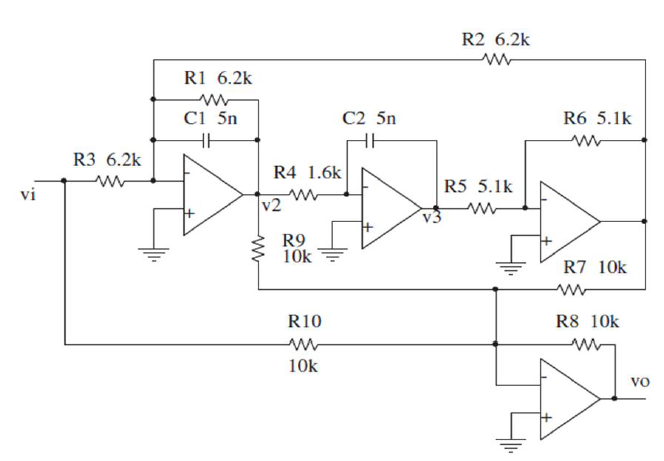
\includegraphics[width=12cm]{./04_Cap4/figures/bickt.png}
\caption{\label{fig:Circuito2}- Circuito: {\textit{Biquad Highpass Filter}}}
\end{center}
\end{figure}

Para simular falhas neste circuito varia-se os valores dos resistores R1, R2, R3 e R4  e dos capacitores C1 e C2.Essa variação esta visível na \ref{tab:falhasckt2}. 

 \begin{table}[H]
         \centering
        \begin{tabular}{ccc}
        \textbf{Grupo} & \textbf{Simulação} & \textbf{Classificação do Erro} \\
        1              & 0-299              & R1 Alto                        \\
        2              & 300-599            & R1 Baixo                       \\
        3              & 600-899            & R2 Alto                        \\
        4              & 900-1199           & R2 Baixo                       \\
        5              & 1200-1499          & R3 Alto                        \\
        6              & 1500-1799          & R3 Baixo                       \\
        7              & 1800-2099          & R4 Alto                      \\
        8              & 2100-2399          & R4 Baixo                       \\
        9              & 2400-2699          & C1 Aberto                      \\
        10             & 2700-2999          & C1 Curto                       \\
        11             & 3000-3299          & C2 Aberto                      \\
        12             & 3300-3599          & C2 Curto                       \\
        13             & 3600-3899         & Normal                        
        \end{tabular}
        \caption{\label{tab:falhasckt2}- Falhas circuito 2}
\end{table}

\item[Circuito III - ] 
\textbf{\textit{CTSV (Continuous-Time State-Variable):}} O filtro universal é um circuito projetado com 3 amplificadores operacionais em sua parte ativa, 7 resistores e 2 capacitores, totalizando 9 componentes passivos e 12 componentes no total. A sua arquitetura é mostrada \ref{fig:Circuito3}. Depois do Sallen-Key, este é um dos principais circuitos utilizados no estudo de detecção de falhas pelos mesmos motivos do Sallen-Key. \cite{lombardi} 

\begin{figure}[H]
\begin{center}
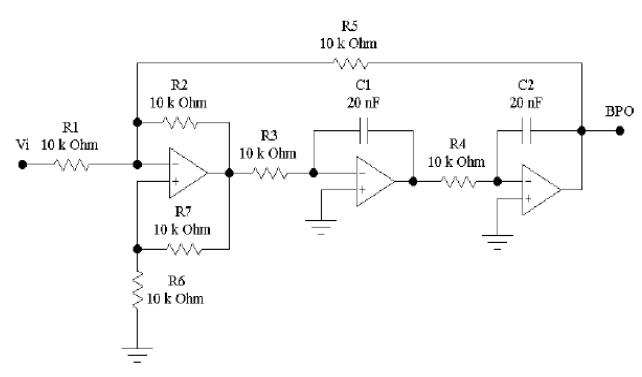
\includegraphics[width=12cm]{./04_Cap4/figures/ctsvckt.png}
\caption{\label{fig:Circuito3}- Circuito: {\textit{ Continuous-Time State-Variable.}}}
\end{center}
\end{figure}

Para simular falhas neste circuito alterna-se os valores dos resistores R1, R2, R3, R4, R5, R6 e R7 e dos capacitores C1 e C2. Essa variação esta visível na \ref{tab:falhasckt3}.
 
 

 \begin{table}[H]
         \centering
        \begin{tabular}{ccc}
        \textbf{Grupo} & \textbf{Simulação} & \textbf{Classificação do Erro} \\
        1              & 0-299              & R1 Alto                        \\
        2              & 300-599            & R2 Baixo                       \\
        3              & 600-899            & R2 Alto                        \\
        4              & 900-1199           & R2 Baixo                       \\
        5              & 1200-1499          & R3 Alto                        \\
        6              & 1500-1799          & R3 Baixo                       \\
        7              & 1800-2099         & R4 Alto                        \\
        8              & 2100-2399          & R4 Baixo                       \\
        9              & 2400-2699          & R5 Alto                        \\
        10             & 2700-2999          & R5 Baixo                       \\
        11             & 3000-3299         & R6 Alto                        \\
        12              & 3300-3599          & R6 Baixo                       \\
        13              & 3600-3899          & R7 Alto                        \\
        14             & 3900-4199          & R7 Baixo                       \\
        15              & 4500-4799         & C1 Aberto                      \\
        16              & 4800-5099         & C1 Curto                       \\
        17              & 5100-5399         & C2 Aberto                      \\
        18               & 5400-5699        & C2 Curto                       \\
        19              & 5700-5999         & Normal                        
        \end{tabular}
        \caption{\label{tab:falhasckt3}- Falhas circuito 3}
\end{table}


\item[Circuito IV - ]\textbf{\textit{ Nonlinear Rectfier:}} Dos 4 circuitos descritos, o retificador não-linear é o único que não é um circuito de filtro e por consequência o circuito mais sensível às variações dos seus parâmetros. A sua arquitetura pode ser vista na \ref{fig:Circuito4}. Não possui componentes ativos e é composta por um único diodo retificador, três capacitores, um indutor e uma resistência \cite{Clayton}.

\begin{figure}[H]
\begin{center}
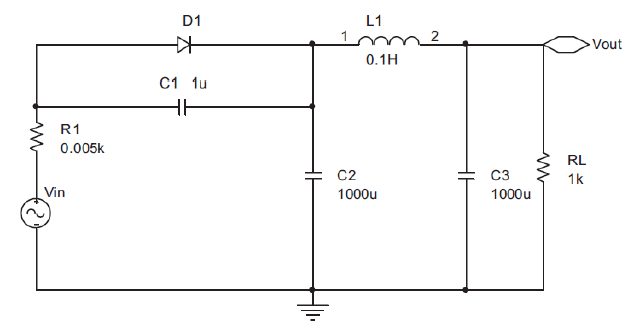
\includegraphics[width=12cm]{./04_Cap4/figures/retificadorckt.png}
\caption{\label{fig:Circuito4}- Circuito:{\textit{ Nonlinear Rectfier}.}}
\end{center}
\end{figure}
Para simular falhas neste circuito provoca-se a variação dos valores dos resistores R1, capacitores C1, C2 e C3 e indutor L1.Essa variação esta visível na \ref{tab:falhasckt4}.

 \begin{table}[H]
         \centering
        \begin{tabular}{ccc}
        \textbf{Grupo} & \textbf{Simulação} & \textbf{Classificação do Erro} \\
        1              & 0-299              & R1 Alto                        \\
        2              & 300-599            & R1 Baixo                       \\
        3              & 600-899            & C1 Aberto                        \\
        4              & 900-1199           & C1 Curto                       \\
        5              & 1200-1499          & C2 Aberto                        \\
        6              & 1500-1799          & C2 Curto                       \\
        7              & 1800-2099          & C3 Aberto                      \\
        8              & 2100-2399          & C3 Curto                       \\
        9              & 2400-2699          & L1 Aberto                      \\
        10             & 2700-2999          & L1 Curto                       \\
        11             & 3000-3299          & Normal                        
        \end{tabular}
        \caption{\label{tab:falhasckt4}- Falhas circuito 4}
\end{table}



\end{enumerate}

Ao simular-se os circuitos segundo parâmetros pré-configurados (tempo de processamento, quantidade de simulações para cada estágio, valores dos componentes, entre outros) a saída dos dados, para todos os nós, é exportada para um arquivo \textit{".raw"}.

\section{\textbf{Leitura dos dados de entrada}}

Para realizar a leitura do arquivo de extensão \textit{".raw"}, exportado pelo LTSpice, é necessário conhecer uma série de instruções sobre os métodos de composição do arquivo. Este arquivo é uma combinação de diferentes estruturas e informações do circuito, armazenadas e comprimidos de modos diferentes.

O desenvolvimento de um processo específico para a leitura deste tipo de arquivo se faz necessário pela falta de uma biblioteca na linguagem que seja destinada especificamente para a leitura de arquivos nativos do LTSpice. 

A primeira linha de qualquer arquivo \textit{".raw"} começará com características da simulação e caminho do sistema, onde se encontra o arquivo de simulação. Por exemplo: 

"
Title: * C:\textbackslash \textbackslash Users\textbackslash \textbackslash jessi\textbackslash \textbackslash PycharmProjects\textbackslash \textbackslash ProjetoFinal\textbackslash \textbackslash Sallen Key mc + 4bitPRBS [FALHA].asc

Date: Wed Jul 25 23:33:14 2018

Plotname: Transient Analysis

Flags: real forward stepped

No. Variables: 42

No. Points:      2943376

Offset:   0.0000000000000000e+000

Command: Linear Technology Corporation LTspice IV

Backannotation: u1 1 2 3 4 5
"


Em seguida o arquivo escreve uma lista com todas as variáveis registradas e armazenadas no circuito. 

Exemplo:

Variables:

	0 & time &	time
	
	1 &	V(clock) &	voltage
	
	2 & 	V(n002) &	voltage
	
	3	V(n004)	voltage
	
	.
	.
	.
	
	40	Ix(u1:4)	subckt_current
	
	41	Ix(u1:5)	subckt_current



A terceira parte do arquivo \textit{".raw"}, finalmente, contém os dados. Eles são armazenados em representação binária e com tamanho proporcional aos dados gerados pela simulação e pelas configurações do programa. Ou seja, existe um alto grau de complexidade para se extrair os dados da simulação e montar um \textit{objeto} (estrutura de dados que lista valores pertinentes a categorizações) devido a incerteza e grande variedade de formato dos dados a serem obtidos. 

Para concluir o processo de aquisição de dados foi usado como base um código ainda incompleto, mas já disponibilizado no \textit{Github} por um desenvolvedor \cite{nuno}, acrescido de várias manipulações de dados. 

Um fator importante a ser destacado é a grande quantidade de dados trabalhada. São processados em torno de 800 milhões de valores ao todo nos quatro circuitos. 


\begin{figure}[H]
\begin{center}
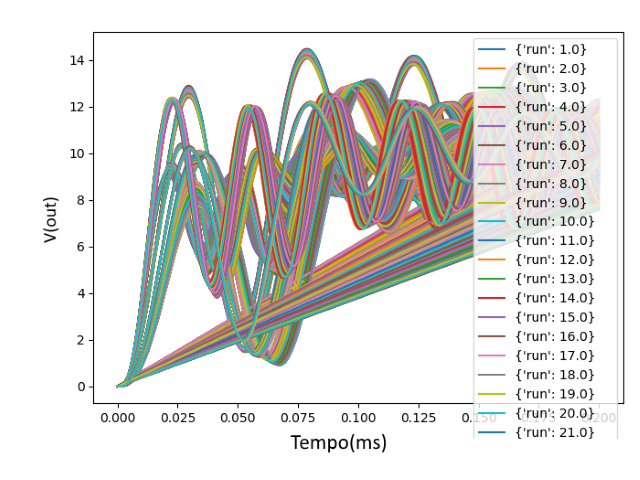
\includegraphics[width=15cm]{./04_Cap4/figures/DadosBrutosNONLinear.png}
\caption{\label{fig:SallenBruto}-Dados Brutos da tensão de saída (Vout x Time)}
\end{center}
\end{figure}


Com os dados inseridos e organizados, foi necessária uma nova etapa: a limpeza e armazenamento dos dados em um CSV. 

Como esse processo de leitura, levando em conta todas as variáveis apresentadas na seção anterior são computacionalmente trabalhosos e demorados, escolheu-se fazer a escrita desses dados em um aquivo CSV para agilizar os testes e compilações posteriores.

Entretanto, para esses dados poderem ser escritos corretamente nas linhas e colunas, preservando os dados desejados e excluindo os valores de variáveis desnecessárias para nosso processo, foi utilizado a técnica de ETL (Extração, transformação e limpeza) \cite{selecao}.

Os dados inicialmente apresentavam, para alguns casos, inconsistências como valores inesperados, formato inadequado, incoerência no relacionamento com a variável tempo, quantidade  diferente de dados para simulações semelhantes entre outros. 

Toda essa manipulação de dados foi desenvolvida utilizando bibliotecas como Pandas e  Numpy, além de bastante manipulação dos dataFrames criados. 

Após esses ajustes e salvando no CSV apenas as variáveis de interesse, conseguimos reduzir os dados para 18 milhões. Só essa alteração já gerou uma grande mudança na velocidade de processamento:  2,25\% dos dados iniciais passam para as próximas fases.
 

\section{\textbf{Extração de Assinaturas (PAA)}}

O passo seguinte foi a aplicação do método de reduzir o numero de dados significativos da simulação. Para isso é usado o PAA (Piecewise Aggregate Approximation – PAA). 

O Aproximação Agregada por Partes (Keogh et al., 2000) é uma técnica de redução de dimensão que é bastante simples de entender e implementar. Ela permite diferentes medidas de distância e apresenta resultados competitivos quando comparada a transformações mais sofisticadas como a decomposição por valor singular (SVD – Singular Value Decomposition) e as Transformadas de Fourier e Wavelet, na tarefa de indexação das séries temporais (Keoghet al., 2000). Uma série temporal (senoidal)
\begin{equation}
X=x_{1},...,x_{n} \end{equation} pode ser representada no espaço N, n \leqslantn ,
\begin{equation}
\overline{X}=\overline{x_{1}},...,\overline{x_{n}}
\end{equation}
\begin{equation}
\overline{x_{i}}= \frac{N}{n}\sum_{j=\frac{N}{n}(i-1)+1}^{\frac{N}{n}i}x_{j}
\end{equation}
A Equação indica que o sinal é dividido em N janelas (segmentos) e que o valor médio representa todos os pontos nesta janela. A \ref{fig:PAASaplicacao} mostra o sinal de uma simulação e sua respectiva representação PAA. O numero de segmentos desejado é uma variável do algoritmo. \cite{timeSerial}. 

\begin{figure}[H]
\begin{center}
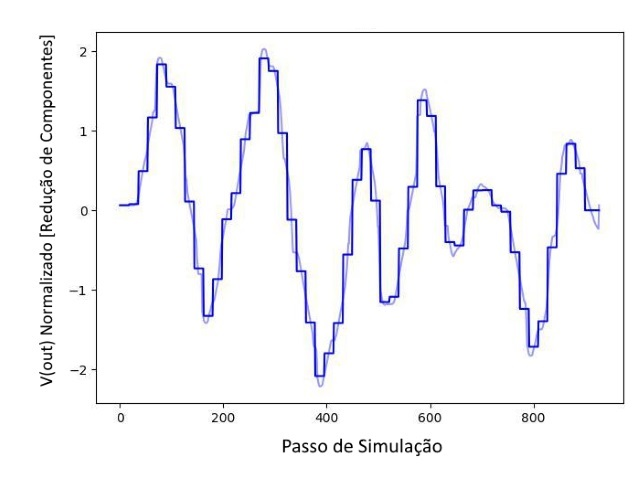
\includegraphics[width=14cm]{./04_Cap4/figures/paa-simples.jpg}
\caption{\label{fig:PAASaplicacao}- Aplicação do PAA (Vout x Time)}
\end{center}
\end{figure}

O método é aplicado a todo DataFrame, diminuindo significamente o número de pontos necessários para representar a simulação e ainda preservar com qualidade o comportamento do modelo. Na \ref{fig:Analisepaa} temos o conjunto de todos os dados de entrada do circuito antes de depois do PAA. Neles há uma redução de 90\% no na variação dos dados, mas mesmo assim eles continuam com o mesmo perfil e agregando bastante dificuldade de os diferenciar, mostrando como o PAA é eficiente ao que se propõe. 

\begin{figure}[H]
\begin{center}
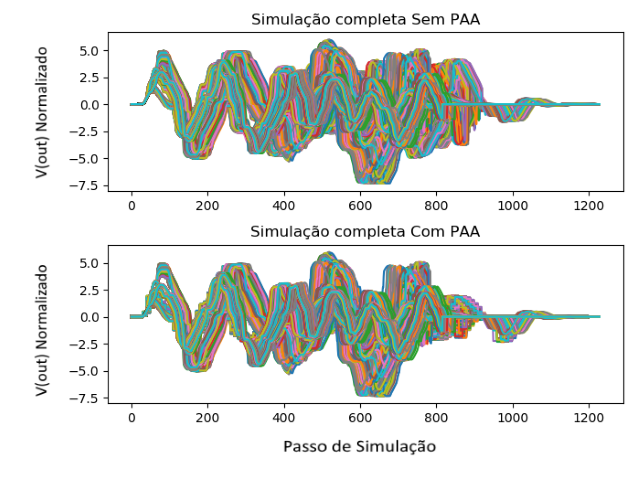
\includegraphics[width=15cm]{./04_Cap4/figures/dadosCompletos.png}
\caption{\label{fig:Analisepaa}- Comparação do Vout antes de depois do PAA (Vout x Time).}
\end{center}
\end{figure}


\section{\textbf{Análise das Componentes Principais (PCA)}}

A Análise das Componentes Principais é a observação do conjunto de dados em um novo espaço, onde este novo conjunto de dados não é linearmente correlacionado. O espaço é definido a partir dos autovalores e autovetores da matriz de covariância dos dados.
Fazendo a covariância das funções no espaço mapeado em x, obtém-se:

\begin{equation}

    {\overline{C}=\frac{1}{n}\sum_{��=1}^{1}\varphi (xi).\varphi (xi)^{T}}
\end{equation}

Temos então que é a matriz de covariância é dada por:

\begin{equation}

\overline{C}=\left[
\begin{array}{c c c}
c_{11}&\ldots& a_{1n}\\
\vdots&\ddots &\vdots\\ c_{n1}&\ldots& c_{nn}
\end{array}\right]

\end{equation}
e
\begin{equation}
c_{ij}=\varphi (xi).\varphi (xi)^{T}

\end{equation}

A aplicação do PCA aconteceu com o auxilio do modulo de PCA da biblioteca sklearn. 


Seguindo seus passos previstos, o PCA base foi calculado através no numero de colunas do dataframe. Esse será por definição o limite de componentes de variância que o método pode ter \cite{pca}. 

Aplica-se um teste para descobrir o numero de componentes necessários para termos uma boa taxa de variância dos dados. 

exemplo do circuito Sallen Key : 

Variância total dos primeiros 1 componentes: 0.38993472912639116

Variância total dos primeiros 2 componentes: 0.6049460165428534

Variância total dos primeiros 3 componentes: 0.7264523762053858

Variância total dos primeiros 4 componentes: 0.8200175327019206

Variância total dos primeiros 5 componentes: 0.8697641955453185

Variância total dos primeiros 6 componentes: 0.8979201818957931

Em seguida insere-se o valor final do número de componentes a serem usados e obtém como resposta os dados reduzidos. 

\begin{figure}[H]
\begin{center}
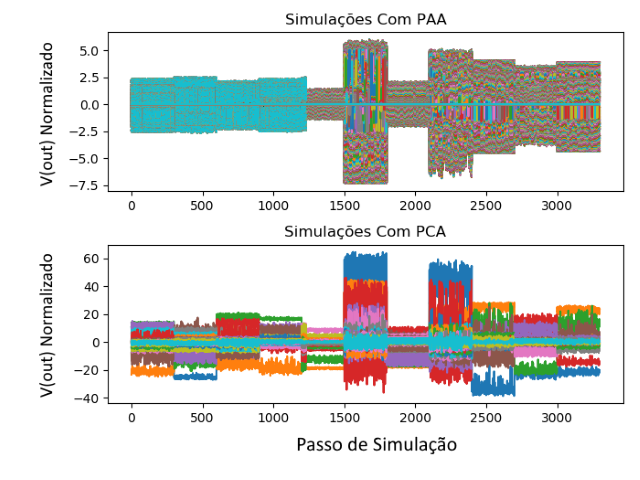
\includegraphics[width=15cm]{./04_Cap4/figures/reducaoPCA.png}
\caption{\label{fig:PCAreducao}- Simulação antes e após o PCA (Vout x Time).}
\end{center}
\end{figure}

Nessa analise é visível como os dados preservam as características, mesmo tendo uma  redução extremamente significativa. O objetivo desse processo de redução é exatamente esse, pegar as principais e mais significativas componentes para as preservar. Essa análise é realizada ao visualizarmos que cada cor significa uma  simulação, a imagem inicial apresenta uma elevada densidade de cores, no segundo caso, essa densidade é diminuída chegando a ter áreas em branco oficializando a redução da quantidade de dados. 

Observando os dados limpos, já é possível perceber diferenças de comportamento para diferentes momentos, já nos aproximando da detecção das falhas. 


\section{\textbf{Aplicação da aprendizagem de maquinas}}

A detecção é realmente realizada nesta etapa do processo. O subsistema consiste basicamente de um classificador e do conjunto de dados processados de características. Antes da real execução da detecção, os dados de resposta do circuito são utilizados para o treinamento do classificador, obtendo o ajuste da sua fronteira de decisão. A seguir, é realizada a detecção para um circuito qualquer, de topologia equivalente aos circuitos treinados. Nesse caso, a saída do classificador corresponderá à saída do sistema de detecção, acusando um determinado defeito ou não no circuito conforme a pertinência do dado obtido à fronteira de decisão do classificador.



Caso desejam-se apenas definir se o circuito apresenta falha ou não, o classificador irá necessitar somente de uma única classe (LI, X., XIE, Y., 2013), não havendo a identificação da falha neste caso. No sistema proposto, é desejado que a detecção não só determine a existência ou não de falha nos circuitos, como também seja capaz de identificá-las. Neste caso, mais classes serão necessárias, havendo N classes de saída para N falhas do circuito.


\begin{figure}[H]
\begin{center}
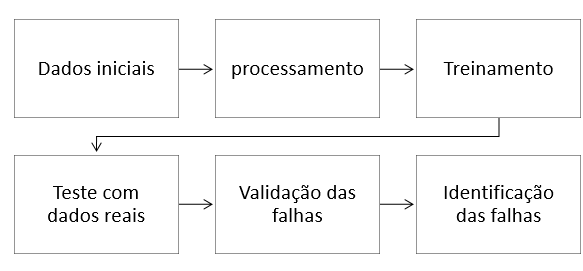
\includegraphics[width=10cm]{./04_Cap4/figures/fluxomachine.PNG}
\caption{\label{fig:fluxomachine}- Diagrama Aprendizado de maquinas}
\end{center}
\end{figure}

A \ref{fig:fluxomachine} exibe o fluxo do dado no processo de aprendizagem. O algoritmo é treinado e depois testado para analisarmos sua taxa de acerto. Após essa etapa, as falhas são identificadas e categorizadas. 

Foram usados 8 algoritmos apresentados no Capitulo 3. Assim podemos diagnosticar quais tem a melhor eficiência para nosso conjunto de dados levando em conta os resultado para os diferentes circuitos. 


\section{\textbf{Validação dos resultados}}

Para avaliar o desempenho dos classificadores primeiro é preciso determinar a porcentagem de falsos positivos e de falsos negativos,ao invés de se analisar apenas a taxa de acerto. Sendo assim, a fração de falsos negativos é definida a priori (fração de rejeição) para a construção do modelo (classificador).
Uma vez que o modelo foi determinado, ele pode ser avaliado em um conjunto de teste e calcular a porcentagem de falsos positivos e falsos negativos. Ainda conforme (Tax, 2008) na literatura existem duas outras medidas que são geralmente usadas: o precision, que é definido na Equação, e o recall, que é basicamente a taxa de verdadeiros positivos e é mostrado na Equação 

\[precision= \text {números de previsões corretas}\div{\text {número de previsões}}\]

\[recall= \text {números de previsões corretas}\div{\text {número de exemplos}}\]


A partir das definições de precision e recall pode-se definir F1 que é uma métrica de
desempenho que está definida na Equação . O F1 relaciona as métricas precision e recall
e essas duas métricas possuem valores no intervalo entre zero e um. Considerando apenas a
relação da multiplicação pela soma do precsion e recall e se os valores forem o máximo, isto
é, precision = 1 e recall =1, o valor máximo dessa relação será 0,5 e com o intuito de
normalizar a métrica F1 = 1, a relação entre o numerador e o denominador é multiplicada por
dois. 

O F1 score foi implementado no algoritmo para nos auxiliar na validação dos resultados\cite{lombardi}. 





%\chapter{Desenvolvimento}

\chapter{Estudo de Caso}

Com o escopo do projeto definido e os conceitos apresentados, podemos apresentar o resultado da implementação. Os testes foram executados para os quatro circuitos descritos: O filtro passa-banda Sallen-Key, o filtro universal (CTSV – Continuous Time State-variable), o filtro passa-alta ativo Biquad (BIQUAD – our Opamp Biquad Highpass Filter) e Retificador não-linear. Os procedimentos para a realização das avaliações são aqueles explicados no capítulo 4, os quais necessitam da obtenção dos conjuntos de treinamento e teste.

Os conjuntos de treinamento e teste são obtidos em duas etapas diferentes. Primeiro, o circuito a ser avaliado é modelado na plataforma de simulação do LTSpice para simulação e modelagem de circuitos eletrônicos.   Sabendo que cada classe de falha apresenta 300 dados contínuos (parâmetro definido) podemos variar o valor do parâmetro (componente) da classe correspondente a cada 300 dados.  Assim um número total de classes de cada circuito de �� = ��300 classes, sendo K a quantidade de falhas pré definidas, falhas no caso é qualquer alteração acima ou abaixo da faixa de tolerância nos componentes do circuito. 

\begin{table}[ht]
\centering
\begin{tabular}{ccc}
\textbf{Circuito}      & \textbf{Nº Falhas} & \textbf{Nº Dados} \\
Filtro Biquadrado      & 12                 & 3900              \\
CSTV                   & 18                 & 6000              \\
Retificador Não linear & 10                 & 3300              \\
Sallen Key             & 10                 & 3300             
\end{tabular}
\caption{\label{tab:resultado}- Falhas dos circuitos}
\end{table}


Na segunda etapa é realizada a transferência dos dados obtidos nas simulações do LTSpice para a leitura em python. Além da dificuldade inicial de realizar a leitura dos dados devido ao modo de construção do arquivo '.raw', foi necessário fazer uma série de validações e manipulações de dados para os deixar em formato pronto para processar.Além disso existia muita informação desnecessária, como a predição aconteceria em relação a Vout, não existe a necessidade de armazenar e manter os dados de medição dos demais nós e componentes do circuito. Esse processo reduziu o volume de dados drasticamente. Após esse processo, os dados são duplicados para termos o conjunto de treino e teste separados.
Uma informação importante a ser destacada são os atributos dos classificadores implementados: DecisionTreeClassifier(random\_state=20);  AdaBoostClassifier(random\_state=20); svm.SVC(kernel='linear', C=1,
random\_state=20); RandomForestClassifier(random\_state=20); GaussianNB(); KNeighborsClassifier(); SGDClassifier(random\_state=20); LogisticRegression(random\_state=20)


\section{\textbf{Sallen Key}}

Usando os códigos que estão anexados no apêndice  foi realizada a aquisição dos dados e tratamento inicial.

 Nas imagens a seguir temos o gráfico do estágio inicial. A  \ref{fig:dadoSalleninicial} exibe os recém adquiridos, mas já manipulado e limpo, ou seja, após o tratamento inicial. 
        
 \begin{figure}[H]
        \begin{center}
        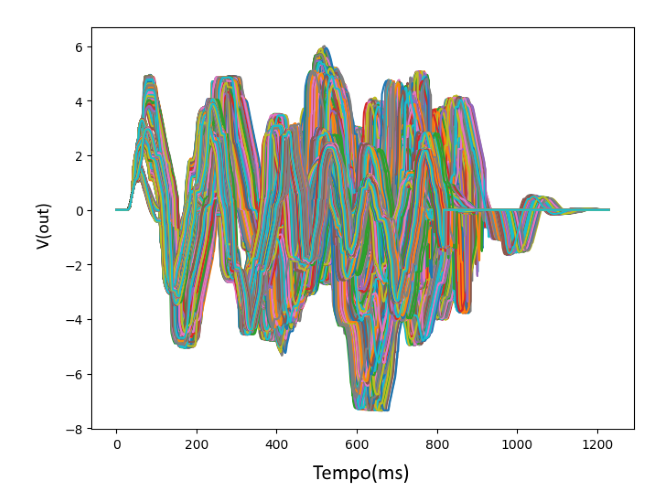
\includegraphics[width=15cm]{./01_Pre_textuais/sallen_figs/dadosPreProc_Sallen_Key_mc_+_4bitPRBS_[FALHA]raw.png}
        \caption{\label{fig:dadoSalleninicial}- Circuito: Sallen key - Dados iniciais (Vout x Time).}
        \end{center}
        \end{figure}
        
Após a aplicação de PAA e PCA temos um conjunto de dados com apenas 5\% dos dados originais. A \ref{fig:pcaSalenkey} exibe os dados limpos e antes de entrar no classificador.

 \begin{figure}[H]
        \begin{center}
        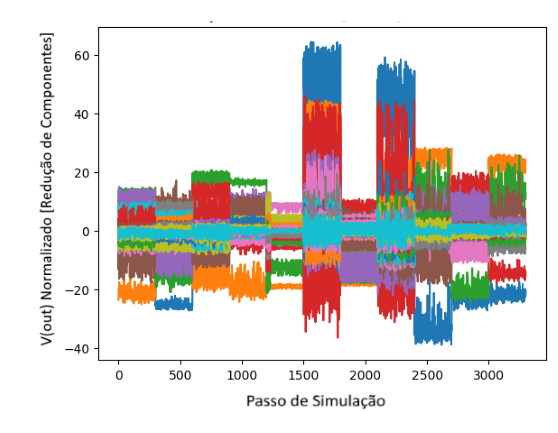
\includegraphics[width=13cm]{./05_Cap5/figures/PCA_Sallen_Key_mc_+_4bitPRBS_[FALHA]raw.png}
        \caption{\label{fig:pcaSalenkey}- Circuito: Sallen key - Dados após processamento (Vout x Time)}
        \end{center}
        \end{figure}

O sistema é classificado com oito métodos diferentes descritos anteriormente e com as falhas determinadas na \ref{tab:falhasckt1}. 

A seguir descrevemos a taxa de acerto para cada um dos algoritmos. 


 
\begin{itemize}
\newpage
 \item Classificador por Árvore de decisão
 
\begin{table}[ht]
\centering
\begin{tabular}{ccc}
\textbf{Classe} & \textbf{Acerto (\%)} & \textbf{Acurácia (\%)} \\
Classe 1        & 100                  & 100                    \\
Classe 2        & 0                  & 0                    \\
Classe 3        & 0                  & 0                    \\
Classe 4        & 0                  & 0                    \\
Classe 5        & 0                  & 0                    \\
Classe 6        & 0                  & 0                    \\
Classe 7        & 0                  & 0                    \\
Classe 8        & 0                  & 0                    \\
Classe 9        & 0                  & 0                    \\
Classe 10       & 0                  & 0                    \\
Classe 11       & 0                  & 0                                       
\end{tabular}
\caption{\label{tab:sallenarvore}- Sallen Key: Falhas Árvore de decisão}
\end{table}

 \begin{figure}[H]
        \begin{center}
       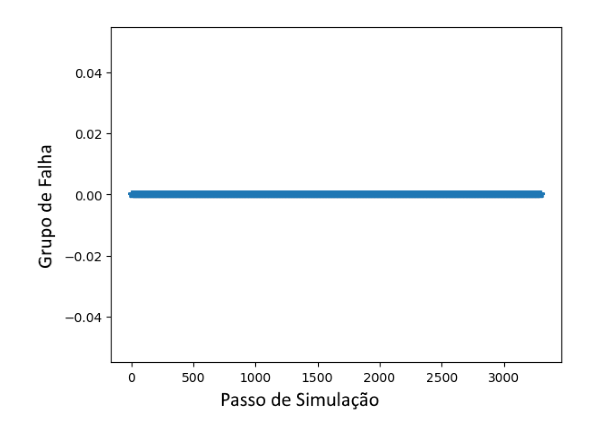
\includegraphics[width=13cm]{./01_Pre_textuais/sallen_figs/DecisionTreeClassifier_Sallen_Key_mc_+_4bitPRBS_[FALHA]raw.png}
        \caption{\label{fig:DecisionTreeClassifieSalenkey}- Circuito: Sallen key - Comportamento da Predição Árvore de decisão}
        \end{center}
        \end{figure}
        
        

A percentual de acerto total é de 9\% para o circuito Sallen Key exemplificado na \ref{fig:DecisionTreeClassifieSalenkey} e \ref{tab:sallenarvore}. 
\newpage
 \item Classificador AdaBoost
 
 \begin{table}[ht]
\centering
\begin{tabular}{ccc}
\textbf{Classe} & \textbf{Acerto (\%)} & \textbf{Acurácia (\%)} \\
Classe 1        & 100                  & 100                    \\
Classe 2        & 100                  & 100                    \\
Classe 3        & 99                  & 99.5                    \\
Classe 4        & 100                  & 100                    \\
Classe 5        & 100                  & 100                    \\
Classe 6        & 100                  & 100                    \\
Classe 7        & 100                  & 100                    \\
Classe 8        & 100                  & 100                    \\
Classe 9        & 100                  & 100                    \\
Classe 10       & 100                  & 100                    \\
Classe 11       & 100                  & 100                               
\end{tabular}
\caption{\label{tab:sallenAdaBoost}- Sallen Key: Falhas AdaBoost}
\end{table}


 \begin{figure}[H]
        \begin{center}
        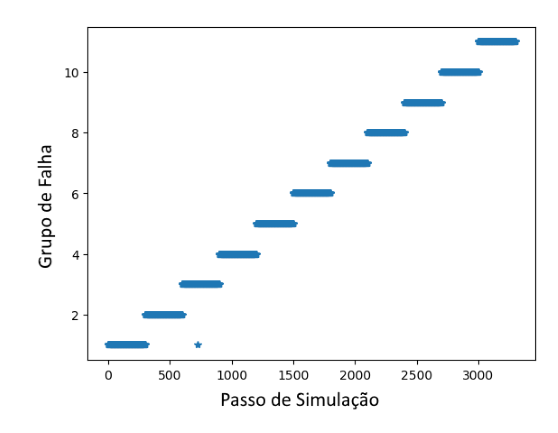
\includegraphics[width=13cm]{./01_Pre_textuais/sallen_figs/AdaBoostClassifier_Sallen_Key_mc_+_4bitPRBS_[FALHA]raw.png}
        \caption{\label{fig:AdaboostClassifieSalenkey}- Circuito: Sallen key - Comportamento da Predição Ada Boost }
        \end{center}
        \end{figure}
       

A percentual de acerto total é de 99,96\% para o circuito Sallen Key exemplificados na \ref{fig:AdaboostClassifieSalenkey} e \ref{tab:sallenAdaBoost}. 

\newpage
 \item Classificador Máquinas de vetores de suporte
 
 \begin{table}[ht]
\centering
\begin{tabular}{ccc}
\textbf{Classe} & \textbf{Acerto (\%)} & \textbf{Acurácia (\%)} \\
Classe 1        & 100                  & 100                    \\
Classe 2        & 0                  & 0                    \\
Classe 3        & 0                  & 0                    \\
Classe 4        & 0                  & 0                    \\
Classe 5        & 0                  & 0                    \\
Classe 6        & 0                  & 0                    \\
Classe 7        & 0                  & 0                    \\
Classe 8        & 98                  & 98                    \\
Classe 9        & 100                  & 100                    \\
Classe 10       & 100                  & 100                    \\
Classe 11       & 0                  & 0                               
\end{tabular}
\caption{\label{tab:sallensvm}- Sallen Key: Falhas SVC}
\end{table}

\begin{figure}[H]
        \begin{center}
        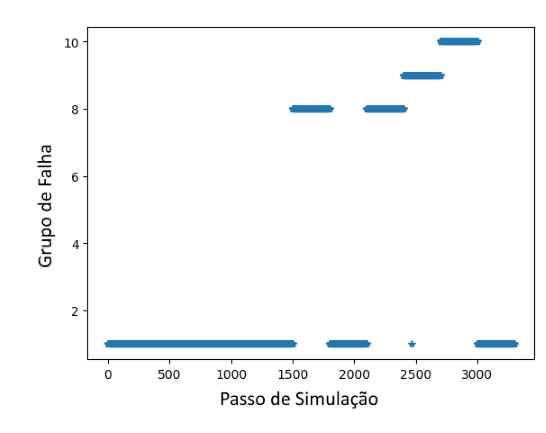
\includegraphics[width=13cm]{./01_Pre_textuais/sallen_figs/SVC_Sallen_Key_mc_+_4bitPRBS_[FALHA]raw.png}
        \caption{\label{fig:SVCClassifieSalenkey}- Circuito: Sallen key - Comportamento da Predição SVC}
        \end{center}
        \end{figure}
       

A percentual de acerto total é de 12,06\% para o circuito Sallen Key exemplificado na \ref{fig:SVCClassifieSalenkey} e \ref{tab:sallensvm}. 

\newpage

 \item Classificador Floresta aleatória
 
 \begin{table}[ht]
\centering
\begin{tabular}{ccc}
\textbf{Classe} & \textbf{Acerto (\%)} & \textbf{Acurácia (\%)} \\
Classe 1        & 100                  & 100                    \\
Classe 2        & 100                  & 100                    \\
Classe 3        & 100                  & 100                    \\
Classe 4        & 100                  & 100                    \\
Classe 5        & 100                  & 100                    \\
Classe 6        & 100                  & 100                    \\
Classe 7        & 100                  & 100                    \\
Classe 8        & 100                  & 100                    \\
Classe 9        & 100                  & 100                    \\
Classe 10       & 100                  & 100                    \\
Classe 11       & 100                  & 100                                  
\end{tabular}
\caption{\label{tab:sallenrandom}- Sallen Key: Falhas Floresta aleatória}
\end{table}


  \begin{figure}[H]
        \begin{center}
        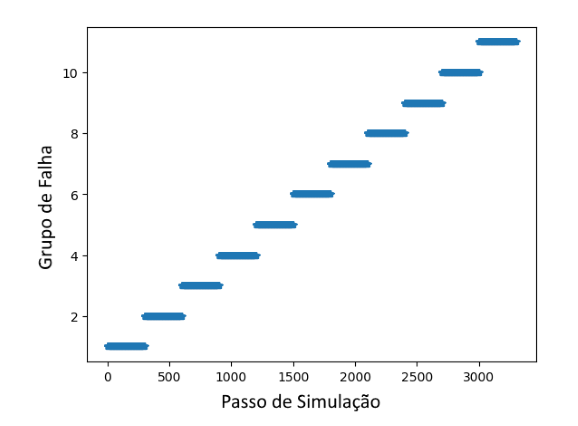
\includegraphics[width=13cm]{./01_Pre_textuais/sallen_figs/RandomForestClassifier_Sallen_Key_mc_+_4bitPRBS_[FALHA]raw.png}
        \caption{\label{fig:randomforestClassifieSalenkey}- Circuito: Sallen key - Comportamento da Predição Random Forest }
        \end{center}
        \end{figure}

A percentual de acerto total é de 100\% para o circuito Sallen Key exemplificado na \ref{fig:randomforestClassifieSalenkey} e \ref{tab:sallenrandom}. 

\newpage
 \item Classificador Gaussiano de Naive Bayes
 
 \begin{table}[ht]
\centering
\begin{tabular}{ccc}
\textbf{Classe} & \textbf{Acerto (\%)} & \textbf{Acurácia (\%)} \\
Classe 1        & 100                  & 100                    \\
Classe 2        & 100                  & 100                    \\
Classe 3        & 98                  & 99                    \\
Classe 4        & 100                  & 100                    \\
Classe 5        & 100                  & 100                    \\
Classe 6        & 100                  & 100                    \\
Classe 7        & 100                  & 100                    \\
Classe 8        & 100                  & 100                    \\
Classe 9        & 100                  & 100                    \\
Classe 10       & 100                  & 100                    \\
Classe 11       & 100                  & 100                                 
\end{tabular}
\caption{\label{tab:sallenGND}- Sallen Key: Falhas Gaussiano de Naive Bayes}
\end{table}


  \begin{figure}[H]
        \begin{center}
        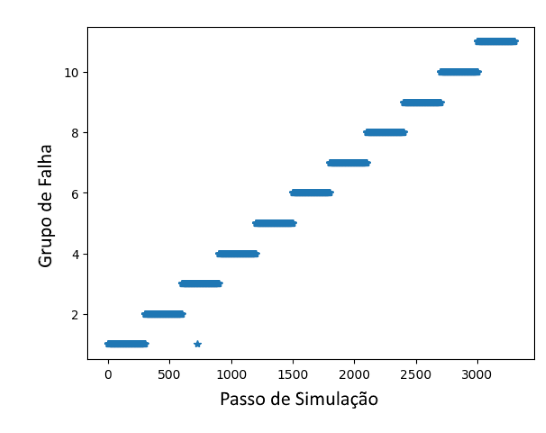
\includegraphics[width=13cm]{./01_Pre_textuais/sallen_figs/GaussianNB_Sallen_Key_mc_+_4bitPRBS_[FALHA]raw.png}
        \caption{\label{fig:GaussianNBClassifieSalenkey}- Circuito: Sallen key - Comportamento Predição GaussianNB}
        \end{center}
        \end{figure}
		
A percentual de acerto total é de 99,87\% para o circuito Sallen Key exemplificado na \ref{fig:GaussianNBClassifieSalenkey} e \ref{tab:sallenGND}. 
\newpage

 \item Classificador K vizinhos mais próximos
 
 \begin{table}[ht]
\centering
\begin{tabular}{ccc}
\textbf{Classe} & \textbf{Acerto (\%)} & \textbf{Acurácia (\%)} \\
Classe 1        & 100                  & 100                    \\
Classe 2        & 100                  & 100                    \\
Classe 3        & 100                  & 100                    \\
Classe 4        & 100                  & 100                    \\
Classe 5        & 100                  & 100                    \\
Classe 6        & 99,9                  & 99,9                    \\
Classe 7        & 100                  & 100                    \\
Classe 8        & 100                  & 100                    \\
Classe 9        & 100                  & 100                    \\
Classe 10       & 100                  & 100                    \\
Classe 11       & 98                  & 98                                 
\end{tabular}
\caption{\label{tab:sallenKvizinhos}- Sallen Key: Falhas K vizinhos}
\end{table}


  \begin{figure}[H]
        \begin{center}
        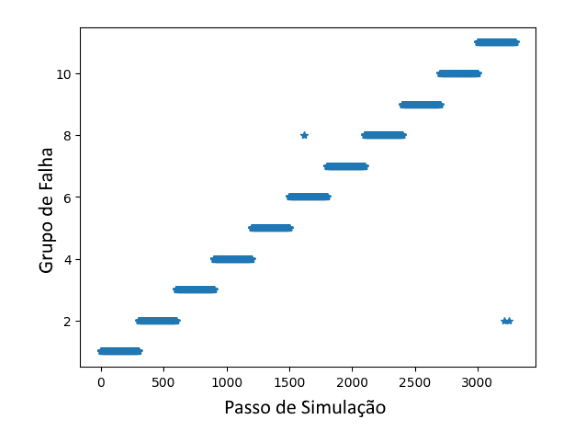
\includegraphics[width=13cm]{./01_Pre_textuais/sallen_figs/KNeighborsClassifier_Sallen_Key_mc_+_4bitPRBS_[FALHA]raw.png}
        \caption{\label{fig:KNeighborsClassifieSalenkey}- Circuito: Sallen key - Comportamento da Predição K Neighbors }
        \end{center}
        \end{figure}

A percentual de acerto total é de 99,8\% para o circuito Sallen Key exemplificado na \ref{fig:KNeighborsClassifieSalenkey} e \ref{tab:sallenKvizinhos}. 
\newpage

 \item Classificador Gradiente de descida estocástica
 
 \begin{table}[ht]
\centering
\begin{tabular}{ccc}
\textbf{Classe} & \textbf{Acerto (\%)} & \textbf{Acurácia (\%)} \\
Classe 1        & 100                  & 100                    \\
Classe 2        & 100                  & 100                    \\
Classe 3        & 100                  & 100                    \\
Classe 4        & 100                  & 100                    \\
Classe 5        & 100                  & 100                    \\
Classe 6        & 100                  & 100                    \\
Classe 7        & 100                  & 100                    \\
Classe 8        & 100                  & 100                    \\
Classe 9        & 100                  & 100                    \\
Classe 10       & 100                  & 100                    \\
Classe 11       & 100                  & 100                                   
\end{tabular}
\caption{\label{tab:sallenGDE}- Sallen Key: Falhas Gradiente de descida estocástica}
\end{table}

 \begin{figure}[H]
        \begin{center}
        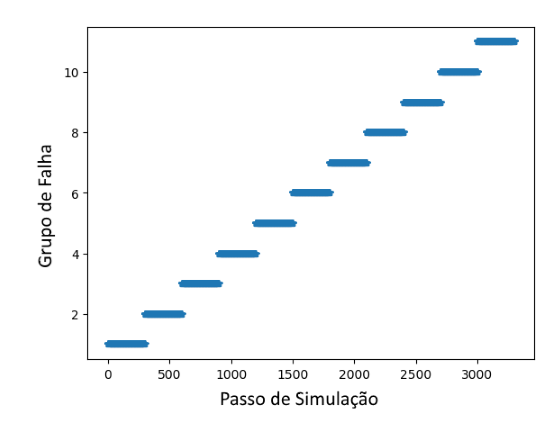
\includegraphics[width=13cm]{./01_Pre_textuais/sallen_figs/SGDClassifier_Sallen_Key_mc_+_4bitPRBS_[FALHA]raw.png}
        \caption{\label{fig:SGDCClassifieSalenkey}- Circuito: Sallen key - Comportamento da Predição SGD}
        \end{center}
        \end{figure}
A percentual de acerto total é de 100\% para o circuito Sallen Key exemplificado na \ref{fig:SGDCClassifieSalenkey} e \ref{tab:sallenGDE}. 

\newpage
 \item Classificador de Regressão logística 
 
 \begin{table}[ht]
\centering
\begin{tabular}{ccc}
\textbf{Classe} & \textbf{Acerto (\%)} & \textbf{Acurácia (\%)} \\
Classe 1        & 100                  & 100                    \\
Classe 2        & 100                  & 100                    \\
Classe 3        & 100                  & 100                    \\
Classe 4        & 100                  & 100                    \\
Classe 5        & 100                  & 100                    \\
Classe 6        & 100                  & 100                    \\
Classe 7        & 100                  & 100                    \\
Classe 8        & 100                  & 100                    \\
Classe 9        & 99                & 99                  \\
Classe 10       & 100                  & 100                    \\
Classe 11       & 100                  & 100                                 
\end{tabular}
\caption{\label{tab:sallenlogistic}- Sallen Key: Falhas Regressão logística}
\end{table}


  \begin{figure}[H]
        \begin{center}
        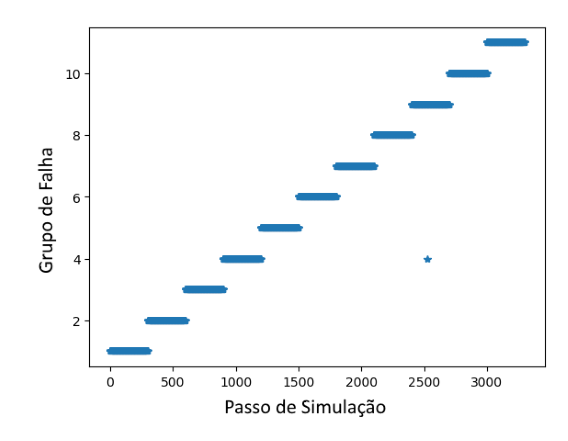
\includegraphics[width=12.5cm]{./01_Pre_textuais/sallen_figs/LogisticRegression_Sallen_Key_mc_+_4bitPRBS_[FALHA]raw.png}
        \caption{\label{fig:LogisticRegressionClassifieSalenkey}- Circuito: Sallen key - Comportamento da Predição regressão Logística }
        \end{center}
        \end{figure}



A percentual de acerto total é de 99,9\% para o circuito Sallen Key exemplificado na \ref{fig:LogisticRegressionClassifieSalenkey} e \ref{tab:sallenlogistic}. 


\end{itemize} 







\section{\textbf{Filtro Passa Alta}}


 Nas imagens a seguir temos o gráfico do estágio inicial. A  \ref{fig:dadobiinicial} exibe os recém adquiridos, mas já manipulado e limpo, ou seja, após o tratamento inicial. 
        
   \begin{figure}[H]
        \begin{center}
        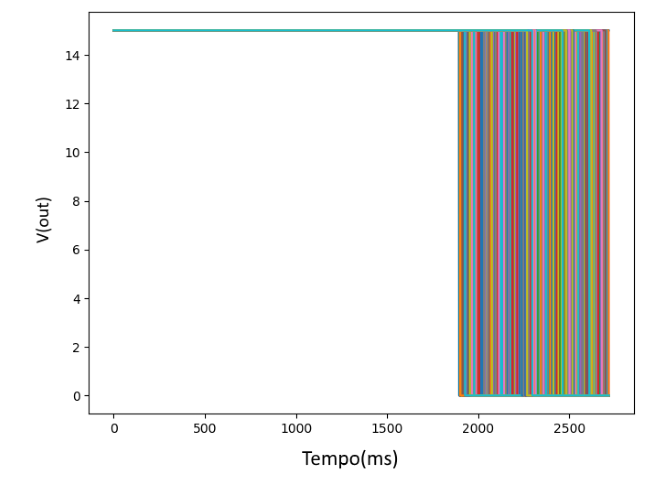
\includegraphics[width=13cm]{./01_Pre_textuais/biquad_figs/dadosPreProc_Biquad_Highpass_Filter_mc_+_4bitPRBS_[FALHA]raw.png}
        \caption{\label{fig:dadobiinicial}- Circuito: Biquad - Dados iniciais}
        \end{center}
        \end{figure}
        
Após a aplicação de PAA e PCA temos um conjunto de dados com apenas 5\% dos dados originais. A \ref{fig:pcabi} exibe os dados limpos e antes de entrar no classificador.

 \begin{figure}[H]
        \begin{center}
        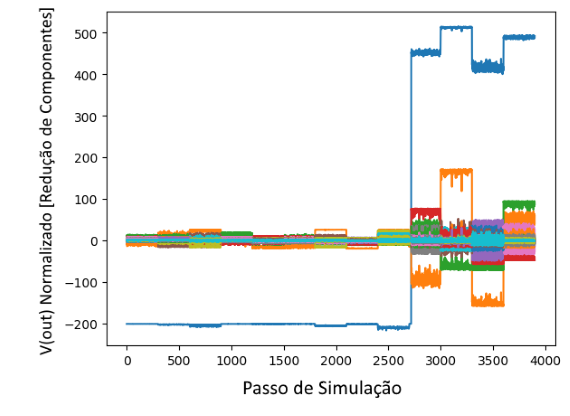
\includegraphics[width=13cm]{./01_Pre_textuais/biquad_figs/PCA_Biquad_Highpass_Filter_mc_+_4bitPRBS_[FALHA]raw.png}
        \caption{\label{fig:pcabi}- Circuito: Biquad - Dados após processamento}
        \end{center}
        \end{figure}
        
O sistema é classificado com oito métodos diferentes descritos anteriormente e com as falhas determinadas na \ref{tab:falhasckt2}. 

A seguir descrevemos a taxa de acerto para cada um dos algoritmos. 


\begin{itemize}
\newpage
 \item Classificador por Árvore de decisão
 
\begin{table}[ht]
\centering
\begin{tabular}{ccc}
\textbf{Classe} & \textbf{Acerto (\%)} & \textbf{Acurácia (\%)} \\
Classe 1        & 100                  & 100                    \\
Classe 2        & 0                  & 0                    \\
Classe 3        & 0                  & 0                    \\
Classe 4        & 0                  & 0                    \\
Classe 5        & 0                  & 0                    \\
Classe 6        & 0                  & 0                    \\
Classe 7        & 0                  & 0                    \\
Classe 8        & 0                  & 0                    \\
Classe 9        & 0                  & 0                    \\
Classe 10       & 0                  & 0                    \\
Classe 11       & 0                  & 0                                       
\end{tabular}
\caption{\label{tab:Biqnarvore}- Biquad: Falhas Árvore de decisão}
\end{table}

 \begin{figure}[H]
        \begin{center}
        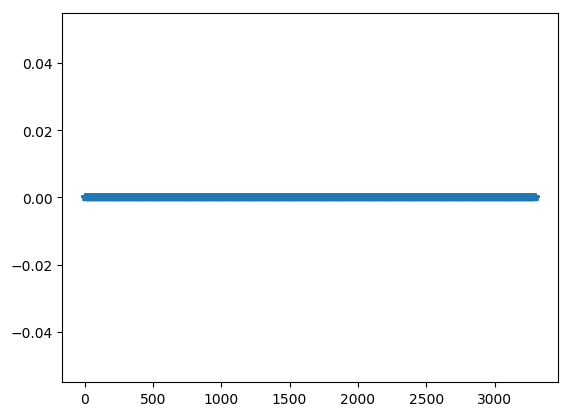
\includegraphics[width=13cm]{./01_Pre_textuais/biquad_figs/DecisionTreeClassifier_Biquad_Highpass_Filter_mc_+_4bitPRBS_[FALHA]raw.png}
        \caption{\label{fig:DecisionTreeClassifieBiq}- Circuito: Biquad - Comportamento da Predição Árvore de decisão}
        \end{center}
        \end{figure}

A percentual de acerto total é de 9\% para o circuito Biquad exemplificado na \ref{fig:DecisionTreeClassifieBiq} e \ref{tab:Biqnarvore}. 
\newpage
 \item Classificador AdaBoost
 
 \begin{table}[ht]
\centering
\begin{tabular}{ccc}
\textbf{Classe} & \textbf{Acerto (\%)} & \textbf{Acurácia (\%)} \\
Classe 1        & 74,2                  & 75                    \\
Classe 2        & 92,42                  & 93                    \\
Classe 3        & 84,69                  & 83,4                    \\
Classe 4        & 62,4                  & 62,4                    \\
Classe 5        & 36,3                  & 36,5                    \\
Classe 6        & 45,4                  & 45,5                    \\
Classe 7        & 93,9                  & 94                    \\
Classe 8        & 99,4                  & 99,5                    \\
Classe 9        & 99,3                 & 99                    \\
Classe 10       & 100                  & 100                    \\
Classe 11       & 100                  & 100                               
\end{tabular}
\caption{\label{tab:BiqnAdaBoost}- Biquad: Falhas AdaBoost}
\end{table}


 \begin{figure}[H]
        \begin{center}
        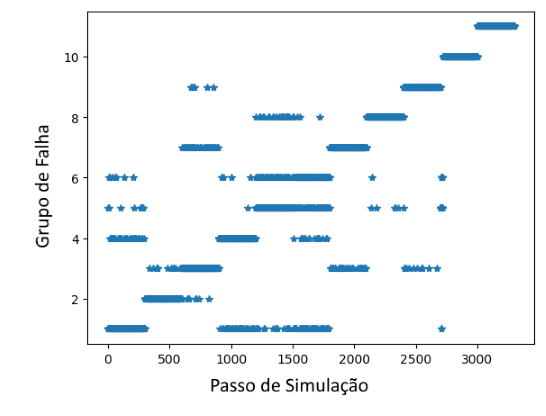
\includegraphics[width=13cm]{./01_Pre_textuais/biquad_figs/AdaBoostClassifier_Biquad_Highpass_Filter_mc_+_4bitPRBS_[FALHA]raw.png}
        \caption{\label{fig:AdaboostClassifieBiq}- Circuito: Biquad - Comportamento da Predição Ada Boost }
        \end{center}
        \end{figure}
       

A percentual de acerto total é de 80,72\% para o circuito Biquad exemplificado na \ref{fig:AdaboostClassifieBiq} e \ref{tab:BiqnAdaBoost}. 

\newpage
 \item Classificador Máquinas de vetores de suporte
 
 \begin{table}[ht]
\centering
\begin{tabular}{ccc}
\textbf{Classe} & \textbf{Acerto (\%)} & \textbf{Acurácia (\%)} \\
Classe 1        & 0                  & 0                    \\
Classe 2        & 0                  & 0                    \\
Classe 3        & 0                  & 0                    \\
Classe 4        & 0                  & 0                    \\
Classe 5        & 0                  & 0                    \\
Classe 6        & 0                  & 0                    \\
Classe 7        & 78,7                  & 79                    \\
Classe 8        & 100                  & 100                    \\
Classe 9        & 0                  & 0                    \\
Classe 10       & 0                  & 0                    \\
Classe 11       & 100                  & 100                               
\end{tabular}
\caption{\label{tab:Biqnsvm}- Biquad: Falhas SVC}
\end{table}

\begin{figure}[H]
        \begin{center}
        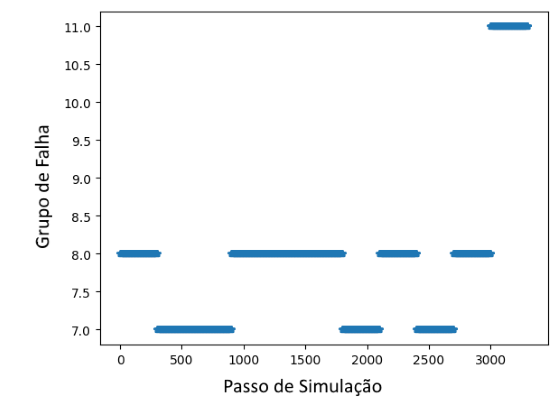
\includegraphics[width=13cm]{./01_Pre_textuais/biquad_figs/SVC_Biquad_Highpass_Filter_mc_+_4bitPRBS_[FALHA]raw.png}
        \caption{\label{fig:SVCClassifieBiq}- Circuito: Biquad - Comportamento da Predição SVC}
        \end{center}
        \end{figure}
       

A percentual de acerto total é de 25,33\% para o circuito Biquad exemplificado na \ref{fig:SVCClassifieBiq} e \ref{tab:Biqnsvm}. 

\newpage

 \item Classificador Floresta aleatória
 
 \begin{table}[ht]
\centering
\begin{tabular}{ccc}
\textbf{Classe} & \textbf{Acerto (\%)} & \textbf{Acurácia (\%)} \\
Classe 1        & 96,7                 & 95,5                   \\
Classe 2        & 77,4                  & 77,4                    \\
Classe 3        & 40,7                  & 40,7                    \\
Classe 4        & 63,6                  & 63,7                    \\
Classe 5        & 34,72                  & 35                    \\
Classe 6        & 44,42                  & 44,5                   \\
Classe 7        & 99,3                  & 99,4                      \\
Classe 8        & 96,9                  & 96,5                 \\
Classe 9        & 100                  & 100                    \\
Classe 10       & 100                  & 100                    \\
Classe 11       & 100                  & 100                                  
\end{tabular}
\caption{\label{tab:Biqnrandom}- Biquad: Falhas Floresta aleatória}
\end{table}


  \begin{figure}[H]
        \begin{center}
        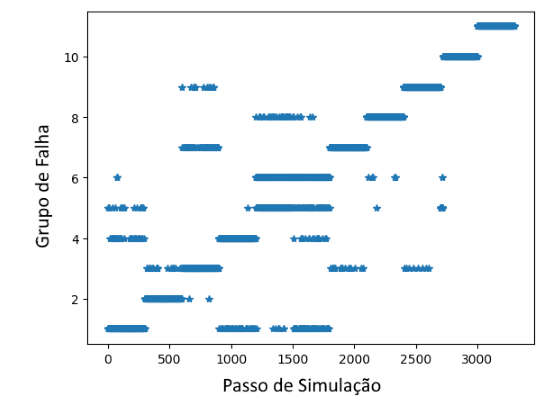
\includegraphics[width=13cm]{./01_Pre_textuais/biquad_figs/RandomForestClassifier_Biquad_Highpass_Filter_mc_+_4bitPRBS_[FALHA]raw.png}
        \caption{\label{fig:randomforestClassifieBiq}- Circuito: Biquad - Comportamento da Predição Random Forest }
        \end{center}
        \end{figure}

A percentual de acerto total é de 77,55\% para o circuito Biquad exemplificado na \ref{fig:randomforestClassifieBiq} e \ref{tab:Biqnrandom}. 

\newpage
 \item Classificador Gaussiano de Naive Bayes
 
 \begin{table}[ht]
\centering
\begin{tabular}{ccc}
\textbf{Classe} & \textbf{Acerto (\%)} & \textbf{Acurácia (\%)} \\
Classe 1        & 76,8                  & 83,9                   \\
Classe 2        & 89,5                  & 97,3                    \\
Classe 3        & 62,8                  & 86,4                    \\
Classe 4        & 83,8                  & 76,5                    \\
Classe 5        & 53,5                  & 83,7                    \\
Classe 6        & 44,42                & 37,8                    \\
Classe 7        & 92,5                  & 74,9                    \\
Classe 8        & 98,9                  & 94,7                    \\
Classe 9        & 98,36            & 99,4                   \\
Classe 10       & 100                  & 99                    \\
Classe 11       & 100                  & 100                                 
\end{tabular}
\caption{\label{tab:BiqnGND}- Biquad: Falhas Gaussiano de Naive Bayes}
\end{table}


  \begin{figure}[H]
        \begin{center}
        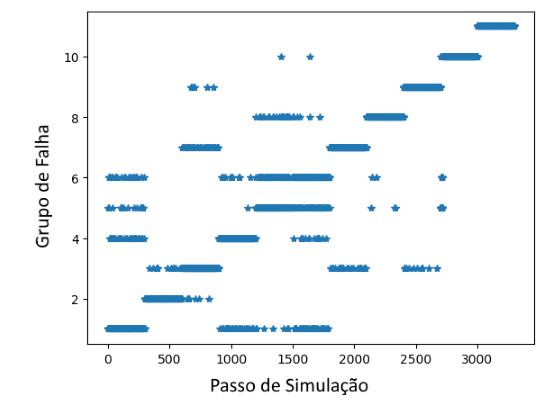
\includegraphics[width=13cm]{./01_Pre_textuais/biquad_figs/GaussianNB_Biquad_Highpass_Filter_mc_+_4bitPRBS_[FALHA]raw.png}
        \caption{\label{fig:GaussianNBClassifieBiq}- Circuito: Biquad - Comportamento Predição GaussianNB}
        \end{center}
        \end{figure}
		
A percentual de acerto total é de 81.87\% para o circuito Biquad exemplificado na \ref{fig:GaussianNBClassifieBiq} e \ref{tab:BiqnGND}. 
\newpage

 \item Classificador K vizinhos mais próximos
 
 \begin{table}[ht]
\centering
\begin{tabular}{ccc}
\textbf{Classe} & \textbf{Acerto (\%)} & \textbf{Acurácia (\%)} \\
Classe 1        & 98                   & 61,8                    \\
Classe 2        & 97,4                  & 91,2                    \\
Classe 3        & 48,6                  & 79,3                    \\
Classe 4        & 56,78                  & 92,4                    \\
Classe 5        & 45,5                  & 98,3                    \\
Classe 6        & 38,2                  & 44,4                    \\
Classe 7        & 97,1                  & 74,2                    \\
Classe 8        & 99,3                  & 96,4                    \\
Classe 9        & 99,6                  & 94,3                    \\
Classe 10       & 100                  & 99,9                    \\
Classe 11       & 99,9                  & 100                                 
\end{tabular}
\caption{\label{tab:BiqnKvizinhos}- Biquad: Falhas K vizinhos}
\end{table}


  \begin{figure}[H]
        \begin{center}
        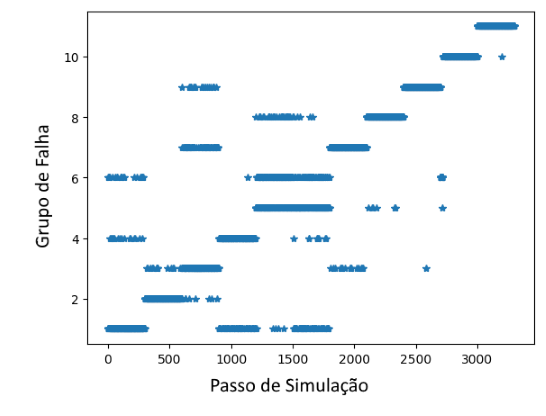
\includegraphics[width=13cm]{./01_Pre_textuais/biquad_figs/KNeighborsClassifier_Biquad_Highpass_Filter_mc_+_4bitPRBS_[FALHA]raw.png}
        \caption{\label{fig:KNeighborsClassifieBiq}- Circuito: Biquad - Comportamento da Predição K Neighbors }
        \end{center}
        \end{figure}

A percentual de acerto total é de 80\% para o circuito Biquad exemplificado na \ref{fig:KNeighborsClassifieBiq} e \ref{tab:BiqnKvizinhos}. 
\newpage

 \item Classificador Gradiente de descida estocástica
 
 \begin{table}[ht]
\centering
\begin{tabular}{ccc}
\textbf{Classe} & \textbf{Acerto (\%)} & \textbf{Acurácia (\%)} \\
Classe 1        & 87,2                  & 91                   \\
Classe 2        & 97,4                  & 99,8                   \\
Classe 3        & 74,8                  & 89,6                    \\
Classe 4        & 64,3                  & 78,8                    \\
Classe 5        & 73,2                  & 94,3                    \\
Classe 6        & 51,4                  & 48,8                    \\
Classe 7        & 98,7                  & 67,4                    \\
Classe 8        & 99,3                  & 84,2                    \\
Classe 9        & 99,5                  & 99,7                    \\
Classe 10       & 100                  & 100                    \\
Classe 11       & 100                  & 100                                   
\end{tabular}
\caption{\label{tab:BiqnGDE}- Biquad: Falhas Gradiente de descida estocástica}
\end{table}

 \begin{figure}[H]
        \begin{center}
        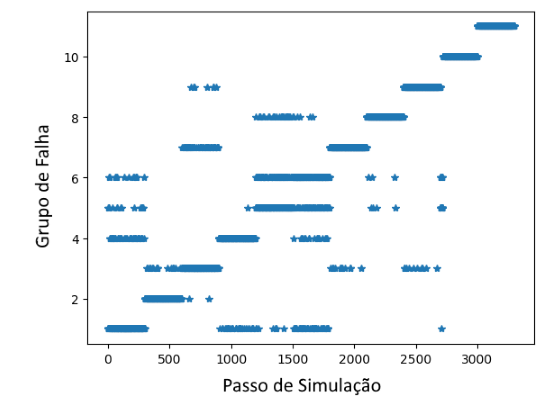
\includegraphics[width=13cm]{./01_Pre_textuais/biquad_figs/SGDClassifier_Biquad_Highpass_Filter_mc_+_4bitPRBS_[FALHA]raw.png}
        \caption{\label{fig:SGDCClassifieBiq}- Circuito: Biquad - Comportamento da Predição SGD}
        \end{center}
        \end{figure}
A percentual de acerto total é de 85,98\% para o circuito Biquad exemplificado na \ref{fig:SGDCClassifieBiq} e \ref{tab:BiqnGDE}. 

\newpage
 \item Classificador de Regressão logística 
 
 \begin{table}[ht]
\centering
\begin{tabular}{ccc}
\textbf{Classe} & \textbf{Acerto (\%)} & \textbf{Acurácia (\%)} \\
Classe 1        & 62,2                  & 86,1                    \\
Classe 2        & 98,3                  & 99,3                    \\
Classe 3        & 36,8                  & 86,2                    \\
Classe 4        & 77,1                  & 51,2                    \\
Classe 5        & 56,8                  & 32,7                    \\
Classe 6        & 0                  & 0                    \\
Classe 7        & 99,8                  & 61,3                   \\
Classe 8        & 99,1                  & 99,8                    \\
Classe 9        & 97                  & 99,6                    \\
Classe 10       & 100                  & 100                    \\
Classe 11       & 100                  & 98,2                                 
\end{tabular}
\caption{\label{tab:Biqnlogistic}- Biquad: Falhas Regressão logística}
\end{table}


  \begin{figure}[H]
        \begin{center}
        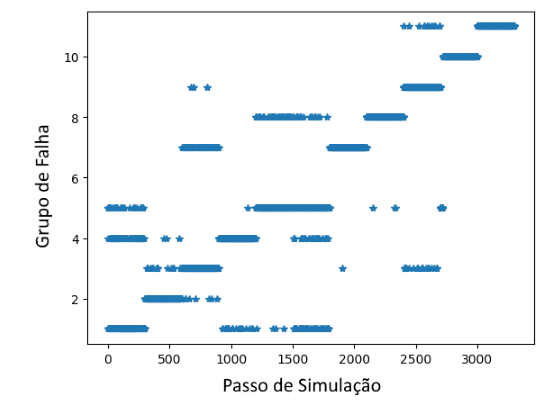
\includegraphics[width=12.5cm]{./01_Pre_textuais/biquad_figs/LogisticRegression_Biquad_Highpass_Filter_mc_+_4bitPRBS_[FALHA]raw.png}
        \caption{\label{fig:LogisticRegressionClassifieBiq}- Circuito: Biquad - Comportamento da Predição regressão Logística }
        \end{center}
        \end{figure}

A percentual de acerto total é de 78,53\% para o circuito Biquad exemplificado na \ref{fig:LogisticRegressionClassifieBiq} e \ref{tab:Biqnlogistic}. 


\end{itemize} 

\section{\textbf{Filtro universal}}


 Nas imagens a seguir temos o gráfico do estágio inicial. A  \ref{fig:dadoCSTVinicial} exibe os recém adquiridos, mas já manipulado e limpo, ou seja, após o tratamento inicial. 
  
  \begin{figure}[H]
        \begin{center}
        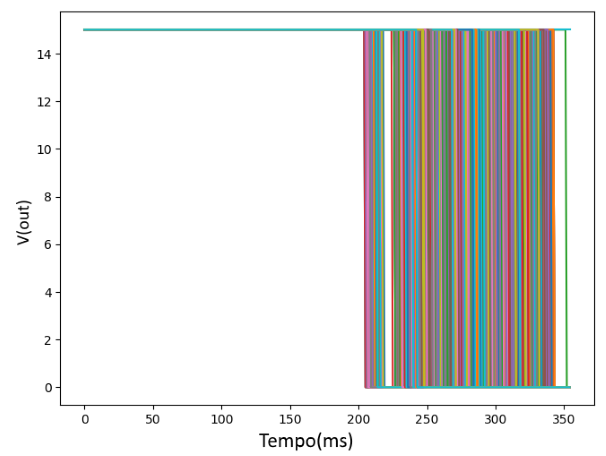
\includegraphics[width=13cm]{./01_Pre_textuais/ctsv_figs/dadosPreProc_CTSV_mc_+_4bitPRBS_[FALHA]raw.png}
        \caption{\label{fig:dadoCSTVinicial}- Circuito: CTSV - Dados iniciais}
        \end{center}
        \end{figure}
        

Após a aplicação de PAA e PCA temos um conjunto de dados com apenas 5\% dos dados originais. A \ref{fig:pcacstv} exibe os dados limpos e antes de entrar no classificador.

\begin{figure}[H]
        \begin{center}
        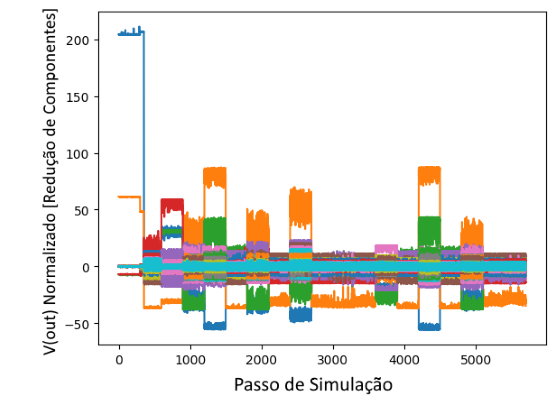
\includegraphics[width=13cm]{./01_Pre_textuais/ctsv_figs/PCA_CTSV_mc_+_4bitPRBS_[FALHA]raw.png}
        \caption{\label{fig:pcacstv}- Circuito: CTSV  - Dados após processamento}
        \end{center}
        \end{figure}

O sistema é classificado com oito métodos diferentes descritos anteriormente e com as falhas determinadas na \ref{tab:falhasckt3}. 

A seguir descrevemos a taxa de acerto para cada um dos algoritmos. 
\newpage

\begin{itemize}

 \item Classificador por Árvore de decisão
 
\begin{table}[ht]
\centering
\begin{tabular}{ccc}
\textbf{Classe} & \textbf{Acerto (\%)} & \textbf{Acurácia (\%)} \\
Classe 1        & 100                  & 5,2                    \\
Classe 2        & 0                 & 0                   \\
Classe 3       & 0                 & 0                     \\
Classe 4       & 0                 & 0                     \\
Classe 5        & 0                 & 0                     \\
Classe 6        & 0                 & 0                      \\
Classe 7        & 0                 & 0                      \\
Classe 8        & 0                 & 0                     \\
Classe 9        & 0                 & 0                     \\
Classe 10       & 0                 & 0                     \\
Classe 11      & 0                 & 0      
     \\
Classe 12       & 0                 & 0   
     \\
Classe 13      & 0                 & 0    
     \\
Classe 14       & 0                 & 0   
     \\
Classe 15       & 0                 & 0    
     \\
Classe 16       & 0                 & 0   
     \\
Classe 17       & 0                 & 0   
     \\
Classe 18     & 0                 & 0    
     \\
Classe 19       & 0                 & 0   
\end{tabular}
\caption{\label{tab:ctsvnarvore}- CTSV: Falhas Árvore de decisão}
\end{table}

 \begin{figure}[H]
        \begin{center}
        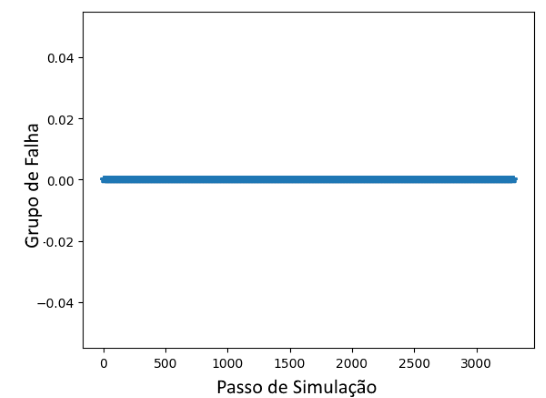
\includegraphics[width=11cm]{./01_Pre_textuais/ctsv_figs/DecisionTreeClassifier_CTSV_mc_+_4bitPRBS_[FALHA]raw.png}
        \caption{\label{fig:DecisionTreeClassifiectsv}- Circuito: CTSV - Comportamento da Predição Árvore de decisão}
        \end{center}
        \end{figure}

A percentual de acerto total é de 5,2\% para o circuito CTSV exemplificado na \ref{fig:DecisionTreeClassifiectsv} e \ref{tab:ctsvnarvore}. 
\newpage
 \item Classificador AdaBoost
 
 \begin{table}[ht]
\centering
\begin{tabular}{ccc}
\textbf{Classe} & \textbf{Acerto (\%)} & \textbf{Acurácia (\%)} \\
Classe 1        & 100                  & 100                    \\
Classe 2        & 95,6                  & 91,2                    \\
Classe 3        & 89,2                  & 100                    \\
Classe 4        & 58,1                  & 62,5                    \\
Classe 5        & 89,2                 & 98,2                    \\
Classe 6        & 63,4                  & 82,7                    \\
Classe 7        & 73,8                  & 48,9                    \\
Classe 8        & 76                  & 39                    \\
Classe 9        & 87                  & 93,9                    \\
Classe 10       & 0                  & 0                    \\
Classe 11       & 75,8            & 100   
     \\
Classe 12       & 0                 & 0   
     \\
Classe 13      & 21,8                 & 12    
     \\
Classe 14       &  75,9                & 56,8   
     \\
Classe 15       & 95                 & 94
     \\
Classe 16       & 52,9                &    76,8
     \\
Classe 17       & 65,9                & 21,7
     \\
Classe 18     &  67,4              &    65,8 
     \\
Classe 19       & 72,8                 & 73,1   
\end{tabular}
\caption{\label{tab:ctsvnAdaBoost}- CTSV: Falhas AdaBoost}
\end{table}


 \begin{figure}[H]
        \begin{center}
        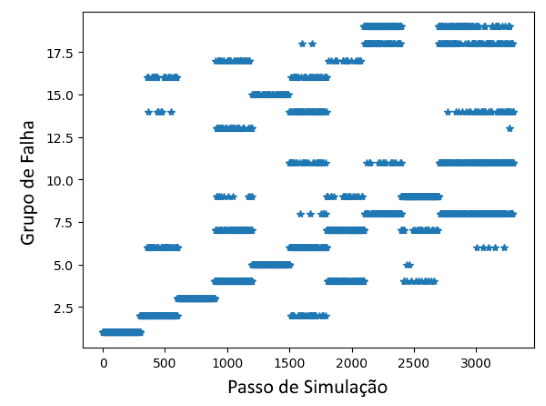
\includegraphics[width=11cm]{./01_Pre_textuais/ctsv_figs/AdaBoostClassifier_CTSV_mc_+_4bitPRBS_[FALHA]raw.png}
        \caption{\label{fig:AdaboostClassifiectsv}- Circuito: CTSV - Comportamento da Predição AdaBoost }
        \end{center}
        \end{figure}
       

A percentual de acerto total é de 66,3\% para o circuito CTSV exemplificado na \ref{fig:AdaboostClassifiectsv} e \ref{tab:ctsvnAdaBoost}. 

\newpage
 \item Classificador Máquinas de vetores de suporte
 
 \begin{table}[ht]
\centering
\begin{tabular}{ccc}
\textbf{Classe} & \textbf{Acerto (\%)} & \textbf{Acurácia (\%)} \\
Classe 1        & 100                  & 100                    \\
Classe 2        & 0                  & 0                    \\
Classe 3        & 100                  & 100                    \\
Classe 4        & 0                  & 0                    \\
Classe 5        & 0                  & 0                    \\
Classe 6        & 0                  & 0                    \\
Classe 7        & 0                  & 0                    \\
Classe 8        & 0                  & 0                    \\
Classe 9        & 100                  & 98                    \\
Classe 10       & 0                  & 0                    \\
Classe 11       & 87                  & 22,4 
\\
Classe 12       & 0                 & 0   
     \\
Classe 13      & 0                 & 0    
     \\
Classe 14       & 0                 & 0   
     \\
Classe 15       & 0                 & 0    
     \\
Classe 16       & 0                 & 0   
     \\
Classe 17       & 0                 & 0   
     \\
Classe 18     & 0                 & 0    
     \\
Classe 19       & 0                 & 0   
\end{tabular}
\caption{\label{tab:ctsvnsvm}- CTSV: Falhas SVC}
\end{table}

\begin{figure}[H]
        \begin{center}
        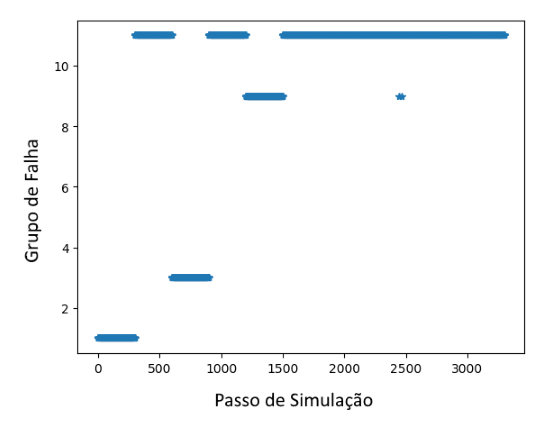
\includegraphics[width=11cm]{./01_Pre_textuais/ctsv_figs/SVC_CTSV_mc_+_4bitPRBS_[FALHA]raw.png}
        \caption{\label{fig:SVCClassifiectsv}- Circuito: CTSV - Comportamento da Predição SVC}
        \end{center}
        \end{figure}
       

A percentual de acerto total é de 20,36\% para o circuito CTSV exemplificado na \ref{fig:SVCClassifiectsv} e \ref{tab:ctsvnsvm}. 

\newpage

 \item Classificador Floresta aleatória
 
 \begin{table}[ht]
\centering
\begin{tabular}{ccc}
\textbf{Classe} & \textbf{Acerto (\%)} & \textbf{Acurácia (\%)} \\
Classe 1        & 100                  & 100                    \\
Classe 2        & 95,6                  & 91,2                    \\
Classe 3        & 86,2                  & 100                    \\
Classe 4        & 58,1                  & 62,5                    \\
Classe 5        & 89,2                 & 98,2                    \\
Classe 6        & 63,4                  & 82,7                    \\
Classe 7        & 73,8                  & 48,9                    \\
Classe 8        & 79.8                  & 39                    \\
Classe 9        & 87                  & 93,9                    \\
Classe 10       & 0                  & 0                    \\
Classe 11       & 79,8            & 100   
     \\
Classe 12       & 0                 & 0   
     \\
Classe 13      & 21,8                 & 12    
     \\
Classe 14       &  75,9                & 56,8   
     \\
Classe 15       & 95                 & 94
     \\
Classe 16       & 52,9                &    76,8
     \\
Classe 17       & 60,3                & 21,7
     \\
Classe 18     &  67,4              &    65,8 
     \\
Classe 19       & 79,8                 & 73,1    

\end{tabular}
\caption{\label{tab:ctsvnrandom}- CTSV: Falhas Floresta aleatória}
\end{table}


  \begin{figure}[H]
        \begin{center}
        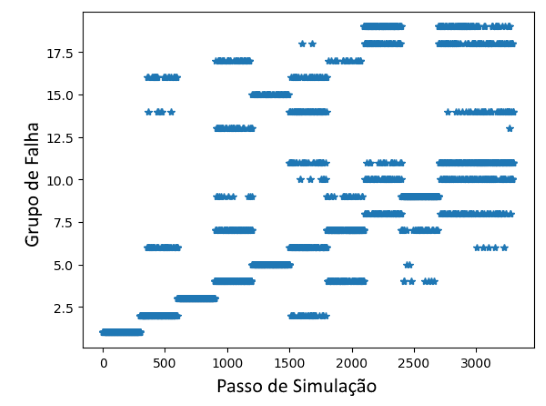
\includegraphics[width=11cm]{./01_Pre_textuais/ctsv_figs/RandomForestClassifier_CTSV_mc_+_4bitPRBS_[FALHA]raw.png}
        \caption{\label{fig:randomforestClassifiectsv}- Circuito: CTSV - Comportamento da Predição Random Forest }
        \end{center}
        \end{figure}

A percentual de acerto total é de 66,63\% para o circuito CTSV exemplificado na \ref{fig:randomforestClassifiectsv} e \ref{tab:ctsvnrandom}. 

\newpage
 \item Classificador Gaussiano de Naive Bayes
 
 \begin{table}[ht]
\centering
\begin{tabular}{ccc}
\textbf{Classe} & \textbf{Acerto (\%)} & \textbf{Acurácia (\%)} \\
Classe 1        & 100                  & 100                    \\
Classe 2        & 95,6                  & 95,2                    \\
Classe 3        & 86,2                  & 100                    \\
Classe 4        & 58,1                  & 67,5                    \\
Classe 5        & 83,2                 & 98,2                    \\
Classe 6        & 63,4                  & 82,7                    \\
Classe 7        & 73,2                  & 48,9                    \\
Classe 8        & 79.8                  & 37,9                    \\
Classe 9        & 82.8                  & 94,9                    \\
Classe 10       & 0                  & 0                    \\
Classe 11       & 81,8            & 89,9   
     \\
Classe 12       & 0                 & 0   
     \\
Classe 13      & 24,8                 & 13,4    
     \\
Classe 14       &  75,9                & 56,8   
     \\
Classe 15       & 93,7                 & 94
     \\
Classe 16       & 59,9                &    76,8
     \\
Classe 17       & 57,3                & 21,7
     \\
Classe 18     &  68,4              &    62,8 
     \\
Classe 19       & 77,8                 & 73,1                                 
\end{tabular}
\caption{\label{tab:ctsvnGND}- CTSV: Falhas Gaussiano de Naive Bayes}
\end{table}


  \begin{figure}[H]
        \begin{center}
        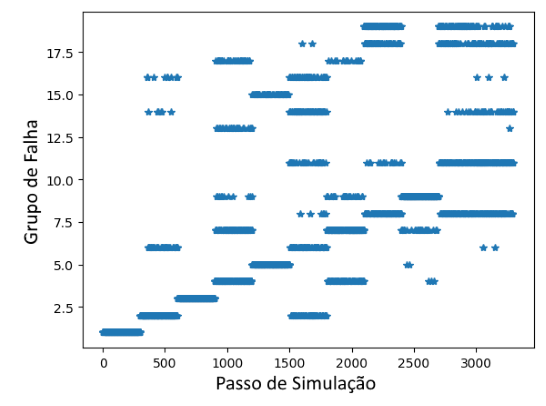
\includegraphics[width=11cm]{./01_Pre_textuais/ctsv_figs/GaussianNB_CTSV_mc_+_4bitPRBS_[FALHA]raw.png}
        \caption{\label{fig:GaussianNBClassifiectsv}- Circuito: CTSV - Comportamento Predição GaussianNB}
        \end{center}
        \end{figure}
		
A percentual de acerto total é de 66,39\% para o circuito CTSV exemplificado na \ref{fig:GaussianNBClassifiectsv} e \ref{tab:ctsvnGND}. 
\newpage

 \item Classificador K vizinhos mais próximos
 
 \begin{table}[ht]
\centering
\begin{tabular}{ccc}
\textbf{Classe} & \textbf{Acerto (\%)} & \textbf{Acurácia (\%)} \\
Classe 1        & 99,8                  & 100                    \\
Classe 2        & 92,6                  & 99,2                    \\
Classe 3        & 86,2                  & 100                    \\
Classe 4        & 0                  & 0                    \\
Classe 5        & 89,8                 & 98,2                    \\
Classe 6        & 68,4                  & 82,7                    \\
Classe 7        & 73,8                  & 48,9                    \\
Classe 8        & 79.8                  & 39                    \\
Classe 9        & 87                  & 93,9                    \\
Classe 10       & 17                  & 76                    \\
Classe 11       & 79,8            & 100   
     \\
Classe 12       & 0                 & 0   
     \\
Classe 13      & 21,8                 & 12    
     \\
Classe 14       &  78,9                & 56,8   
     \\
Classe 15       & 56                 & 94
     \\
Classe 16       & 76,9                &    76,8
     \\
Classe 17       & 19,3                & 21,7
     \\
Classe 18     &  42,4              &    65,8 
     \\
Classe 19       & 39,8                 & 73,1                                
\end{tabular}
\caption{\label{tab:ctsvnKvizinhos}- CTSV: Falhas K vizinhos}
\end{table}


  \begin{figure}[H]
        \begin{center}
        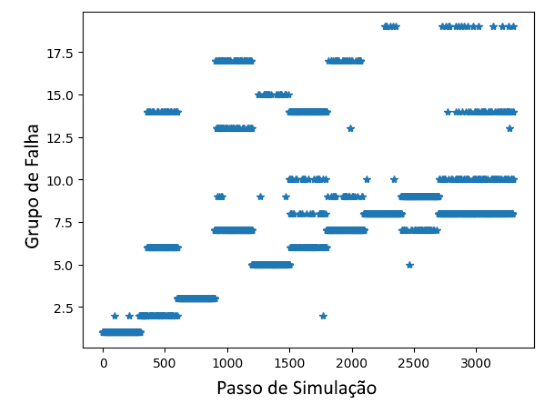
\includegraphics[width=11cm]{./01_Pre_textuais/ctsv_figs/KNeighborsClassifier_CTSV_mc_+_4bitPRBS_[FALHA]raw.png}
        \caption{\label{fig:KNeighborsClassifiectsv}- Circuito: CTSV - Comportamento da Predição K Neighbors }
        \end{center}
        \end{figure}

A percentual de acerto total é de 58,38\% para o circuito CTSV exemplificado na \ref{fig:KNeighborsClassifiectsv} e \ref{tab:ctsvnKvizinhos}. 
\newpage

 \item Classificador Gradiente de descida estocástica
 
 \begin{table}[ht]
\centering
\begin{tabular}{ccc}
\textbf{Classe} & \textbf{Acerto (\%)} & \textbf{Acurácia (\%)} \\
Classe 1        & 100                  & 100                    \\
Classe 2        & 68,6                  & 56,2                    \\
Classe 3        & 86,2                  & 100                    \\
Classe 4        & 78,1                  & 62,5                    \\
Classe 5        & 89,2                 & 98,2                    \\
Classe 6        & 63,4                  & 82,7                    \\
Classe 7        & 73,8                  & 87,9                    \\
Classe 8        & 79.8                  & 89                    \\
Classe 9        & 67.9                  & 93,9                    \\
Classe 10       & 0                  & 0                    \\
Classe 11       & 88,8            & 76   
     \\
Classe 12       & 67,9                 & 85,4   
     \\
Classe 13      & 21,8                 & 12    
     \\
Classe 14       &  75,9                & 56,8   
     \\
Classe 15       & 95                 & 94
     \\
Classe 16       & 52,9                &    76,8
     \\
Classe 17       & 60,3                & 21,7
     \\
Classe 18     &  57,4              &    65,8 
     \\
Classe 19       & 59,8                 & 73,1                                   
\end{tabular}
\caption{\label{tab:ctsvnGDE}- CTSV: Falhas Gradiente de descida estocástica}
\end{table}

 \begin{figure}[H]
        \begin{center}
        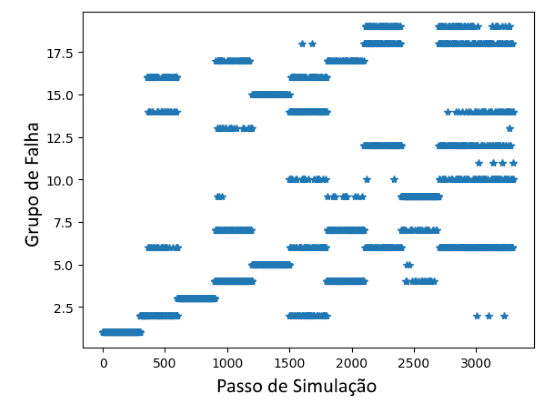
\includegraphics[width=11cm]{./01_Pre_textuais/ctsv_figs/SGDClassifier_CTSV_mc_+_4bitPRBS_[FALHA]raw.png}
        \caption{\label{fig:SGDCClassifiectsv}- Circuito: CTSV - Comportamento da Predição SGD}
        \end{center}
        \end{figure}
A percentual de acerto total é de 84,98\% para o circuito CTSV exemplificado na \ref{fig:SGDCClassifiectsv} e \ref{tab:ctsvnGDE}. 

\newpage
 \item Classificador de Regressão logística 
 
 \begin{table}[ht]
\centering
\begin{tabular}{ccc}
\textbf{Classe} & \textbf{Acerto (\%)} & \textbf{Acurácia (\%)} \\
Classe 1        & 97,5                  & 93,7                    \\
Classe 2        & 85,6                  & 91,2                    \\
Classe 3        & 96,2                  & 100                    \\
Classe 4        & 58,1                  & 62,5                    \\
Classe 5        & 94,2                 & 99,2                    \\
Classe 6        & 76,4                  & 59,7                    \\
Classe 7        & 0                  & 0                    \\
Classe 8        & 0                  & 0                    \\
Classe 9        & 87                  & 93,9                    \\
Classe 10       & 0                  & 0                    \\
Classe 11       & 64,5            & 32,5   
     \\
Classe 12       & 67                 & 75   
     \\
Classe 13      & 21,8                 & 65    
     \\
Classe 14       &  77,9                & 56,8   
     \\
Classe 15       & 95                 & 94
     \\
Classe 16       & 0                &    0
     \\
Classe 17       & 86,3                & 67,7
     \\
Classe 18     &  0              &    0 
     \\
Classe 19       & 0                 & 0                                 
\end{tabular}
\caption{\label{tab:ctsvnlogistic}- CTSV: Falhas Regressão logística}
\end{table}


  \begin{figure}[H]
        \begin{center}
        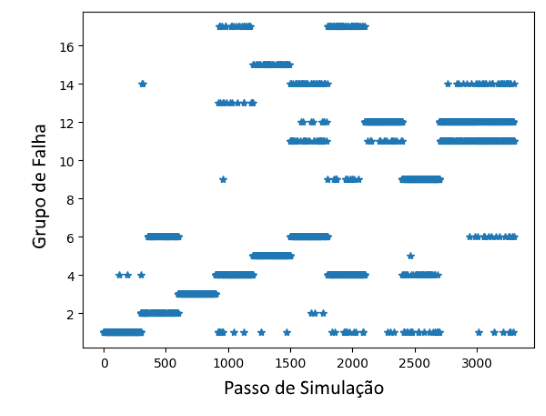
\includegraphics[width=11cm]{./01_Pre_textuais/ctsv_figs/LogisticRegression_CTSV_mc_+_4bitPRBS_[FALHA]raw.png}
        \caption{\label{fig:LogisticRegressionClassifiectsv}- Circuito: CTSV - Comportamento da regressão Logística }
        \end{center}
        \end{figure}

A percentual de acerto total é de 53,02\% para o circuito CTSV exemplificado na \ref{fig:LogisticRegressionClassifiectsv} e \ref{tab:ctsvnlogistic}. 


\end{itemize} 


\section{\textbf{Retificador não linear}}


 Nas imagens a seguir temos o gráfico do estágio inicial. A  \ref{fig:dadoPAAretificador} exibe os recém adquiridos, mas já manipulado e limpo, ou seja, após o tratamento inicial. 
 
\begin{figure}[H]
        \begin{center}
        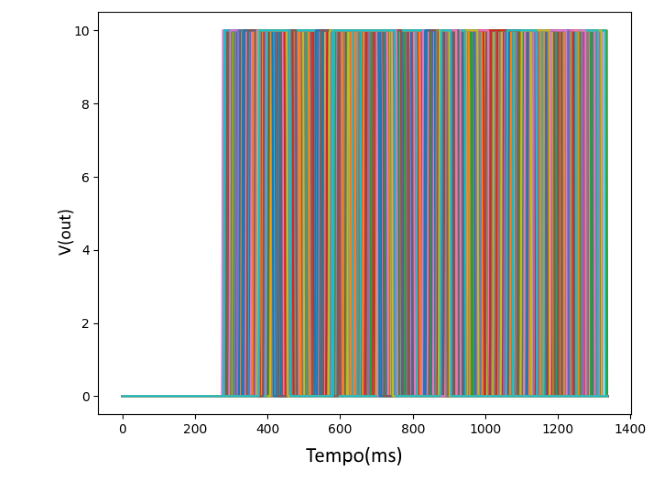
\includegraphics[width=13cm]{./01_Pre_textuais/nonlin_figs/dadosPreProc_Nonlinear_Rectfier_+_4bit_PRBS_[FALHA]_-_300_-_02sraw.png}
        \caption{\label{fig:dadoPAAretificador}- Circuito: Retificador  - Dados iniciais}
        \end{center}
        \end{figure}
        
Após a aplicação de PAA e PCA temos um conjunto de dados com apenas 5\% dos dados originais. A \ref{fig:pcaretificador} exibe os dados limpos e antes de entrar no classificador.

\begin{figure}[H]
        \begin{center}
        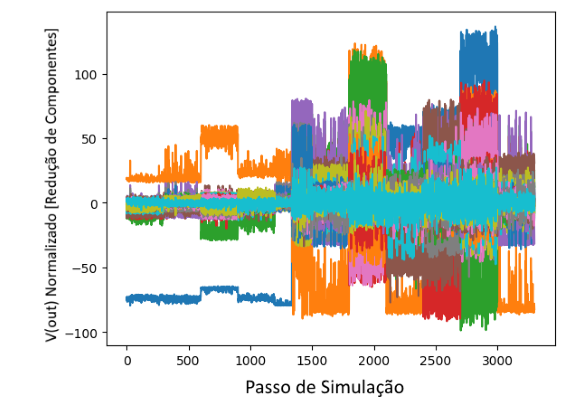
\includegraphics[width=13cm]{./01_Pre_textuais/nonlin_figs/PCA_Nonlinear_Rectfier_+_4bit_PRBS_[FALHA]_-_300_-_02sraw.png}
        \caption{\label{fig:pcaretificador}- Circuito: Retificador - Dados após processamento}
        \end{center}
        \end{figure}

O sistema é classificado com oito métodos diferentes descritos anteriormente e com as falhas determinadas na \ref{tab:falhasckt4}. 

A seguir descrevemos a taxa de acerto para cada um dos algoritmos. 


\begin{itemize}
\newpage
 \item Classificador por Árvore de decisão
 
\begin{table}[ht]
\centering
\begin{tabular}{ccc}
\textbf{Classe} & \textbf{Acerto (\%)} & \textbf{Acurácia (\%)} \\
Classe 1        & 100                  & 9                    \\
Classe 2         & 0                  & 0                    \\
Classe 3        & 0                  & 0                     \\
Classe 4       & 0                  & 0                     \\
Classe 5        & 0                  & 0                    \\
Classe 6        & 0                  & 0                     \\
Classe 7         & 0                  & 0                     \\
Classe 8         & 0                  & 0                      \\
Classe 9         & 0                  & 0                     \\
Classe 10        & 0                  & 0                    \\
Classe 11       & 0                  & 0                                      
\end{tabular}
\caption{\label{tab:Retnarvore}- Retificador: Falhas Árvore de decisão}
\end{table}

 \begin{figure}[H]
        \begin{center}
        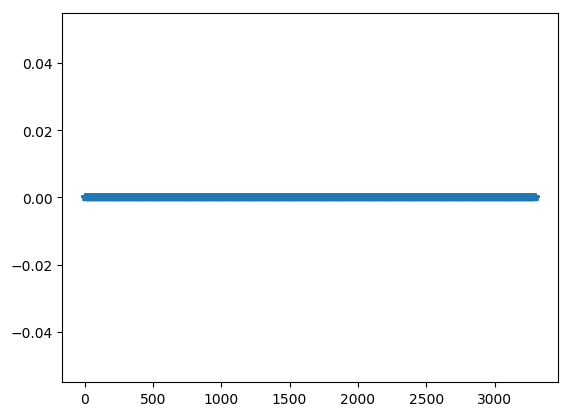
\includegraphics[width=13cm]{./01_Pre_textuais/nonlin_figs/DecisionTreeClassifier_Nonlinear_Rectfier_+_4bit_PRBS_[FALHA]_-_300_-_02sraw.png}
        \caption{\label{fig:DecisionTreeClassifieRet}- Circuito: Retificador - Comportamento da Predição Árvore de decisão}
        \end{center}
        \end{figure}

A percentual de acerto total é de 9\% para o circuito Retificador exemplificado na \ref{fig:DecisionTreeClassifieRet} e \ref{tab:Retnarvore}. 
\newpage
 \item Classificador AdaBoost
 
 \begin{table}[ht]
\centering
\begin{tabular}{ccc}
\textbf{Classe} & \textbf{Acerto (\%)} & \textbf{Acurácia (\%)} \\
Classe 1        & 99,9                  & 99,75                    \\
Classe 2        & 99,84                  & 99,6                    \\
Classe 3        & 100                  & 100                    \\
Classe 4        & 99,87                  & 99,9                    \\
Classe 5        & 99,9                  & 99,8                    \\
Classe 6        & 97,6                  & 97,5                    \\
Classe 7        & 100                  & 100                    \\
Classe 8        & 99,89                  & 99,9                    \\
Classe 9        & 99,9                  & 99,9                    \\
Classe 10       & 99,8                  & 100                    \\
Classe 11       & 98,6                  & 97,6                               
\end{tabular}
\caption{\label{tab:RetnAdaBoost}- Retificador: Falhas AdaBoost}
\end{table}


 \begin{figure}[H]
        \begin{center}
        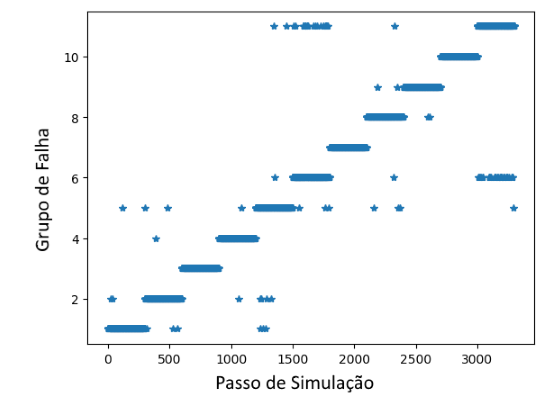
\includegraphics[width=13cm]{./01_Pre_textuais/nonlin_figs/AdaBoostClassifier_Nonlinear_Rectfier_+_4bit_PRBS_[FALHA]_-_300_-_02sraw.png}
        \caption{\label{fig:AdaboostClassifieRet}- Circuito: Retificador - Comportamento da Predição Ada Boost }
        \end{center}
        \end{figure}
       

A percentual de acerto total é de 99,57\% para o circuito Retificador exemplificado na \ref{fig:AdaboostClassifieRet} e \ref{tab:RetnAdaBoost}. 

\newpage
 \item Classificador Máquinas de vetores de suporte
 
 \begin{table}[ht]
\centering
\begin{tabular}{ccc}
\textbf{Classe} & \textbf{Acerto (\%)} & \textbf{Acurácia (\%)} \\
Classe 1        & 100                  & 25,25                    \\
Classe 2        & 0                  & 0                    \\
Classe 3        & 100                  & 100                    \\
Classe 4        & 0                  & 0                    \\
Classe 5        & 0                  & 0                    \\
Classe 6        & 0                  & 0                    \\
Classe 7        & 0                  & 0                    \\
Classe 8        & 0                  & 0                    \\
Classe 9        & 100                  & 36,8                   \\
Classe 10       & 0                  & 0                    \\
Classe 11       & 0                  &  0                              
\end{tabular}
\caption{\label{tab:Retnsvm}- Retificador: Falhas SVC}
\end{table}

\begin{figure}[H]
        \begin{center}
        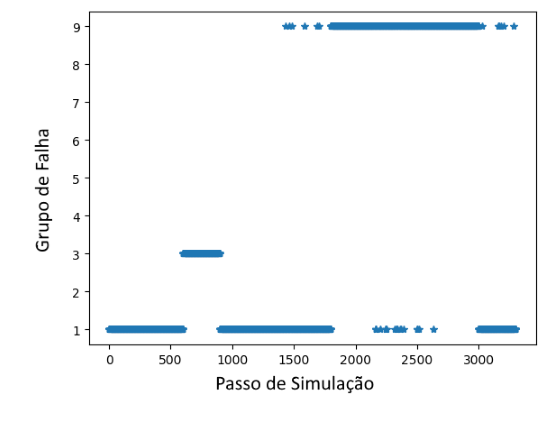
\includegraphics[width=13cm]{./01_Pre_textuais/nonlin_figs/SVC_Nonlinear_Rectfier_+_4bit_PRBS_[FALHA]_-_300_-_02sraw.png}
        \caption{\label{fig:SVCClassifieRet}- Circuito: Retificador - Comportamento da Predição SVC}
        \end{center}
        \end{figure}
       

A percentual de acerto total é de 27,27\% para o circuito Retificador exemplificado na \ref{fig:SVCClassifieRet} e \ref{tab:Retnsvm}. 

\newpage

 \item Classificador Floresta aleatória
 
 \begin{table}[ht]
\centering
\begin{tabular}{ccc}
\textbf{Classe} & \textbf{Acerto (\%)} & \textbf{Acurácia (\%)} \\
Classe 1        & 100                  & 99,9                    \\
Classe 2        & 99,9                  & 99,9                    \\
Classe 3        & 100                  & 100                    \\
Classe 4        & 99,9                  & 100                    \\
Classe 5        & 99,8                  & 99,9                    \\
Classe 6        & 97,4                  & 98,3                    \\
Classe 7        & 98,4                  & 100                    \\
Classe 8        & 99,3                  & 100                    \\
Classe 9        & 100                  & 99,7                    \\
Classe 10       & 99,9                  & 100                    \\
Classe 11       & 97,4                  & 96,5                                  
\end{tabular}
\caption{\label{tab:Retnrandom}- Retificador: Falhas Floresta aleatória}
\end{table}


  \begin{figure}[H]
        \begin{center}
        \includegraphics[width=13cm]{./01_Pre_textuais/nonlin_figs/RandomForestClassifier_Nonlinear_Rectfier_+_4bit_PRBS_[FALHA]_-_300_-_02sraw.png}
        \caption{\label{fig:randomforestClassifieRet}- Circuito: Retificador - Comportamento da Predição Random Forest }
        \end{center}
        \end{figure}

A percentual de acerto total é de 99,27\% para o circuito Retificador exemplificado na \ref{fig:randomforestClassifieRet} e \ref{tab:Retnrandom}. 

\newpage
 \item Classificador Gaussiano de Naive Bayes
 
 \begin{table}[ht]
\centering
\begin{tabular}{ccc}
\textbf{Classe} & \textbf{Acerto (\%)} & \textbf{Acurácia (\%)} \\
Classe 1        & 99,9                  & 99,9                    \\
Classe 2        & 99,9                  & 99,2                    \\
Classe 3        & 100                  & 100                    \\
Classe 4        & 99,8                  & 100                    \\
Classe 5        & 99,9                  & 99,7                    \\
Classe 6        & 98,2                  & 93,7                    \\
Classe 7        & 99,9                  & 100                    \\
Classe 8        & 99,9                  & 99,9                    \\
Classe 9        & 100                  & 99,9                    \\
Classe 10       & 100                  & 100                    \\
Classe 11       & 93,6                  & 97,3                                 
\end{tabular}
\caption{\label{tab:RetnGND}- Retificador: Falhas Gaussiano de Naive Bayes}
\end{table}


  \begin{figure}[H]
        \begin{center}
        \includegraphics[width=13cm]{./01_Pre_textuais/nonlin_figs/GaussianNB_Nonlinear_Rectfier_+_4bit_PRBS_[FALHA]_-_300_-_02sraw.png}
        \caption{\label{fig:GaussianNBClassifieRet}- Circuito: Retificador - Comportamento Predição GaussianNB}
        \end{center}
        \end{figure}
		
A percentual de acerto total é de 99,19\% para o circuito Retificador exemplificado na \ref{fig:GaussianNBClassifieRet} e \ref{tab:RetnGND}. 
\newpage

 \item Classificador K vizinhos mais próximos
 
\begin{table}[ht]
\centering
\begin{tabular}{ccc}
\textbf{Classe} & \textbf{Acerto (\%)} & \textbf{Acurácia (\%)} \\
Classe 1        & 76,2                  & 68,7                    \\
Classe 2        & 78,2                  & 67                    \\
Classe 3        & 96,5                  & 100                    \\
Classe 4        & 85                  & 98,9                    \\
Classe 5        & 62,7                  & 93,2                    \\
Classe 6        & 76,9                  & 88,5                    \\
Classe 7        & 89,9                  & 100                    \\
Classe 8        & 95,6                  & 56,1                    \\
Classe 9        & 74,2                  & 99,7                    \\
Classe 10       & 99,3                  & 100                    \\
Classe 11       & 87,2                  & 64,3                                 
\end{tabular}
\caption{\label{tab:RetnKvizinhos}- Retificador: Falhas K vizinhos}
\end{table}


  \begin{figure}[H]
        \begin{center}
        \includegraphics[width=13cm]{./01_Pre_textuais/nonlin_figs/KNeighborsClassifier_Nonlinear_Rectfier_+_4bit_PRBS_[FALHA]_-_300_-_02sraw.png}
        \caption{\label{fig:KNeighborsClassifieRet}- Circuito: Retificador - Comportamento da Predição K Neighbors }
        \end{center}
        \end{figure}

A percentual de acerto total é de 83,79\% para o circuito Retificador exemplificado na \ref{fig:KNeighborsClassifieRet} e \ref{tab:RetnKvizinhos}. 
\newpage

 \item Classificador Gradiente de descida estocástica
 
 \begin{table}[ht]
\centering
\begin{tabular}{ccc}
\textbf{Classe} & \textbf{Acerto (\%)} & \textbf{Acurácia (\%)} \\
Classe 1        & 99.9                  & 99.8                    \\
Classe 2        & 99.8                  & 100                    \\
Classe 3        & 100                  & 100                    \\
Classe 4        & 100                  & 100                    \\
Classe 5        & 100                  & 97,8                    \\
Classe 6        & 85,4                  & 92,3                    \\
Classe 7        & 97                  & 100                    \\
Classe 8        & 98,3                  & 98,4                    \\
Classe 9        & 97,5                  & 99,9                    \\
Classe 10       & 99                  & 100                    \\
Classe 11       & 87                  & 84                                   
\end{tabular}
\caption{\label{tab:RetnGDE}- Retificador: Falhas Gradiente de descida estocástica}
\end{table}

 \begin{figure}[H]
        \begin{center}
        \includegraphics[width=13cm]{./01_Pre_textuais/nonlin_figs/SGDClassifier_Nonlinear_Rectfier_+_4bit_PRBS_[FALHA]_-_300_-_02sraw.png}
        \caption{\label{fig:SGDCClassifieRet}- Circuito: Retificador - Comportamento da Predição SGD}
        \end{center}
        \end{figure}
A percentual de acerto total é de 96,7\% para o circuito Retificador exemplificado na \ref{fig:SGDCClassifieRet} e \ref{tab:RetnGDE}. 

\newpage
 \item Classificador de Regressão logística 
 
 \begin{table}[ht]
\centering
\begin{tabular}{ccc}
\textbf{Classe} & \textbf{Acerto (\%)} & \textbf{Acurácia (\%)} \\
Classe 1        & 84,7                  & 99,7                    \\
Classe 2        & 91,3                  & 100                    \\
Classe 3        & 99,1                  & 100                    \\
Classe 4        & 99,6                  & 65,2                    \\
Classe 5        & 96,3                  & 76,4                    \\
Classe 6        & 81,2                  & 93.1                    \\
Classe 7        & 100                  & 100                    \\
Classe 8        & 91,3                  & 86                    \\
Classe 9        & 97,3                  & 98,2                    \\
Classe 10       & 99,5               & 99,7                    \\
Classe 11       & 97,3                  & 61                                 
\end{tabular}
\caption{\label{tab:Retnlogistic}- Retificador: Falhas Regressão logística}
\end{table}


  \begin{figure}[H]
        \begin{center}
        \includegraphics[width=12.5cm]{./01_Pre_textuais/nonlin_figs/LogisticRegression_Nonlinear_Rectfier_+_4bit_PRBS_[FALHA]_-_300_-_02sraw.png}
        \caption{\label{fig:LogisticRegressionClassifieRet}- Circuito: Retificador - Comportamento da Predição regressão Logística }
        \end{center}
        \end{figure}

A percentual de acerto total é de 94,32\% para o circuito Retificador exemplificado na \ref{fig:LogisticRegressionClassifieRet} e \ref{tab:Retnlogistic}. 
\end{itemize} 



\label{chapter:exemplo}

\section{\textbf{Resultados}}
Com todos os circuitos simulados, limpos, processados e com sua predição realizada, é possível analisar e comparar os melhores resultados. 

O resultado da predição foi verificado, e então calculado o percentual de acerto de cada um dos algoritmos para cada um dos circuitos. A quantidade percentual de acertos é exibida na \ref{tab:resultadoFinal}.

\begin{table}[H]
\centering
\begin{tabular}{cccccc}
\textbf{Algoritmo}     & \textbf{Circuito 1} & \textbf{Circuito 2} & \textbf{Circuito 3} & \textbf{Circuito 4} & \textbf{Média Acerto}           \\
\textbf{Arvore de D.}  & 9\%                 & 9\%                 & 5,2\%               & 9\%                 & 8,05\%                          \\
\textbf{AdaBoost}      & 99,96\%             & 80,72\%             & 66,3\%              & 99,57\%             & 86,63\% \\
\textbf{SVC}           & 12,06\%             & 25,33\%             & 20,36\%             & 27,27\%             & 21,25\%                         \\
\textbf{Floresta Ale.} & 100\%               & 77,55\%             & 66,63\%             & 99,27\%             & 85,86\%                         \\
\textbf{Naive Bayes}   & 99,87\%             & 81,87\%             & 66,39\%             & 99,19\%             & 86,83\% \\
\textbf{K vizinhos}    & 99,8\%              & 80\%                & 58,38\%             & 83,79\%             & 80,49\%                         \\
\textbf{GDE}           & 100\%               & 84,98\%             & 67,72\%             & 96,7\%              &86,8\%  \\
\textbf{Regressão L.}  & 99,96\%             & 78,53\%             & 53,02\%             & 94,32\%             & 60,20\%                        
\end{tabular}
\caption{\label{tab:resultadoFinal}- Comparação de desempenhos}
\end{table}


Através dos resultados exibidos na \ref{tab:resultadoFinal}, é possível verificar os algoritmos que melhor possuem o melhor desempenho nos diferentes tipos de circuitos. Devido a complexidade dos dados, os classificadores mais robustos obtiveram um melhor desempenho. O circuito 3 (CTSV), que possui uma maior quantidade de falhas e uma topologia mais elaborada, apresentou a maior dificuldade de ser classificado.

Os Algoritmos AdaBoost, Floresta Aleatória e o Gradiente de descida estocástica (GDE), apresentaram os melhores desempenhos sendo 86,63\%, 85,86\% e 86,83\% respectivamente. Importante destacar que alguns deles chegaram a atingir 100\% de acerto na classificação para alguns circuitos. 

Num passo a mais, foi testado a predição unindo os melhores resultados possíveis, ou seja, AdaBoost com estimador base de floresta aleatória. Esse conjunto apresentou uma taxa de acerto de quase 100\% para todos os circuitos.

%\noindent\textbf{CONCLUSÃO}
$\!$\\



O desenvolvimento de estratégias de teste para detectar e diagnosticar falhas em
circuitos analógicos e de sinais mistos é uma tarefa complexa. Existem muitos fatores que
contribuem para o aumento da dificuldade no teste destes circuitos tais como: a necessidade de alterar conexões para medir correntes, a falta de bons modelos de falha, a falta de um
padrão para projeto de circuitos analógicos com vistas a testabilidade e a crescente
importância das falhas temporais. Além disso, os métodos clássicos necessitam de grande
poder computacional se a identificação de parâmetros for utilizada ou caso haja um grande número
de simulações, como no caso de um dicionário de falhas.

Esse desafio tem estimulado o desenvolvimento de ferramentas que buscam facilitar
os procedimentos de detecção de falhas. Em particular o uso de técnicas de Inteligência
Computacional tem sido amplamente empregado, sobretudo através da utilização de
classificadores para identificação de componentes defeituosos.

Este trabalho apresentou um sistema de detecção de falhas para circuitos lineares utilizando  oito diferentes algoritmos de aprendizagem de máquinas. Esse algoritmos foram escolhidos devido sua recorrência na literatura científica. No processo de classificação foram elaboradas algumas etapas: Simulação dos circuitos, extração e limpeza do dados, processamento de redução de dimensão para finalmente o conjunto de treino ser submetido ao algoritmo de classificação e finalizando com a predição com o conjunto de teste. 

Os quatro diferentes circuitos utilizados são o Sallen key, Filtro Passa Alta (Biquad), Filtro universal (CTSV) e o retificador não linear. Os métodos de limpeza e redução foram o PAA e PCA, além de técnicas de ETL com Pandas. 

O resultado da predição foi verificado, e então calculado o percentual de acerto de cada um dos algoritmos para cada um dos circuitos. A quantidade percentual de acertos é exibida na \ref{tab:resultadoFinal}.

Após uma analise geral podemos afirmar quais métodos apresentam uma boa taxa de acerto ou não. Para trabalhos futuros a arvore de decisão por exemplo não precisa ser testado, pois sua ineficiência já foi comprovada.  Em contrapartida, o AdaBoost com o floresta aleatória apresenta uma predição tão elevada que o valida como sendo o melhor do trabalho em questão e o ideal a ser reaplicado em evoluções futuras. 


% Please add the following required packages to your document preamble:
% \usepackage[table,xcdraw]{xcolor}
% If you use beamer only pass "xcolor=table" option, i.e. \documentclass[xcolor=table]{beamer}













% inserir demais capítulos aqui
% -----------------------------
% -----------------------------
% -----------------------------
% -----------------------------





\pagebreak
\addcontentsline{toc}{chapter}{\hspace{1.7cm}\bfseries CONCLUSÃO}
\noindent\textbf{CONCLUSÃO}
$\!$\\



O desenvolvimento de estratégias de teste para detectar e diagnosticar falhas em
circuitos analógicos e de sinais mistos é uma tarefa complexa. Existem muitos fatores que
contribuem para o aumento da dificuldade no teste destes circuitos tais como: a necessidade de alterar conexões para medir correntes, a falta de bons modelos de falha, a falta de um
padrão para projeto de circuitos analógicos com vistas a testabilidade e a crescente
importância das falhas temporais. Além disso, os métodos clássicos necessitam de grande
poder computacional se a identificação de parâmetros for utilizada ou caso haja um grande número
de simulações, como no caso de um dicionário de falhas.

Esse desafio tem estimulado o desenvolvimento de ferramentas que buscam facilitar
os procedimentos de detecção de falhas. Em particular o uso de técnicas de Inteligência
Computacional tem sido amplamente empregado, sobretudo através da utilização de
classificadores para identificação de componentes defeituosos.

Este trabalho apresentou um sistema de detecção de falhas para circuitos lineares utilizando  oito diferentes algoritmos de aprendizagem de máquinas. Esse algoritmos foram escolhidos devido sua recorrência na literatura científica. No processo de classificação foram elaboradas algumas etapas: Simulação dos circuitos, extração e limpeza do dados, processamento de redução de dimensão para finalmente o conjunto de treino ser submetido ao algoritmo de classificação e finalizando com a predição com o conjunto de teste. 

Os quatro diferentes circuitos utilizados são o Sallen key, Filtro Passa Alta (Biquad), Filtro universal (CTSV) e o retificador não linear. Os métodos de limpeza e redução foram o PAA e PCA, além de técnicas de ETL com Pandas. 

O resultado da predição foi verificado, e então calculado o percentual de acerto de cada um dos algoritmos para cada um dos circuitos. A quantidade percentual de acertos é exibida na \ref{tab:resultadoFinal}.

Após uma analise geral podemos afirmar quais métodos apresentam uma boa taxa de acerto ou não. Para trabalhos futuros a arvore de decisão por exemplo não precisa ser testado, pois sua ineficiência já foi comprovada.  Em contrapartida, o AdaBoost com o floresta aleatória apresenta uma predição tão elevada que o valida como sendo o melhor do trabalho em questão e o ideal a ser reaplicado em evoluções futuras. 


% Please add the following required packages to your document preamble:
% \usepackage[table,xcdraw]{xcolor}
% If you use beamer only pass "xcolor=table" option, i.e. \documentclass[xcolor=table]{beamer}












\pagebreak
\addcontentsline{toc}{chapter}{\hspace{1.7cm}\bfseries REFERÊNCIAS}
\def\bibname{REFERÊNCIAS}
\bibliography{dissertacao}

\pagebreak
\addcontentsline{toc}{chapter}{\hspace{1.7cm}\bfseries APÊNDICES}
\def\bibname{APÊNDICES}
\pagebreak
\graphicspath{ {./01_Pre_textuais/code/} }
\DeclareGraphicsExtensions{.png,.pdf}



\appendix


    Apêndice - Códigos desenvolvidos no projeto
    \begin{itemize}
        \item Leitura do Arquivo \textit{.raw}
    \end{itemize}

\begin{figure}[H]
\centering
\includegraphics[scale=0.75]{01_Pre_textuais/code/leitura1.pdf}
\end{figure}
\newpage

\begin{figure}[H]
\centering
\includegraphics[scale=0.9]{01_Pre_textuais/code/leitura2.pdf}
\end{figure}


\begin{figure}[H]
\centering
\includegraphics[scale=0.9]{01_Pre_textuais/code/leitura3.pdf}
\end{figure}
\begin{figure}[H]
\centering
\includegraphics[scale=0.9]{01_Pre_textuais/code/leitura4.pdf}
\end{figure}
\begin{figure}[]
\centering
\includegraphics[scale=0.9]{01_Pre_textuais/code/leitura5.pdf}
\end{figure}
\begin{figure}[]
\centering
\includegraphics[scale=0.9]{01_Pre_textuais/code/leitura6.pdf}
\end{figure}
\begin{figure}[]
\centering
\includegraphics[scale=0.9]{01_Pre_textuais/code/leitura7.pdf}
\end{figure}
\begin{figure}[]
\centering
\includegraphics[scale=0.9]{01_Pre_textuais/code/leitura8.pdf}
\end{figure}
\begin{figure}[]
\centering
\includegraphics[scale=0.9]{01_Pre_textuais/code/leitura9.pdf}
\end{figure}
\begin{figure}[]
\centering
\includegraphics[scale=0.9]{01_Pre_textuais/code/leitura10.pdf}
\end{figure}

\begin{figure}[]
\centering
\includegraphics[scale=0.9]{01_Pre_textuais/code/leitura11.pdf}
\end{figure}

\begin{figure}[]
\centering
\includegraphics[scale=0.9]{01_Pre_textuais/code/leitura12.pdf}
\end{figure}
\begin{figure}[]
\centering
\includegraphics[scale=0.9]{01_Pre_textuais/code/leitura13.pdf}
\end{figure}

\newpage
\begin{itemize}
    \item Criação do Arquivo CSV \textit{.raw}
\end{itemize}

\begin{figure}[H]
\centering
\includegraphics[scale=0.75]{01_Pre_textuais/code/CargaCsv.pdf}
\end{figure}

\newpage

\begin{itemize}
    \item Função com os algoritmos implementados
\end{itemize}
\begin{figure}[H]
\centering
\includegraphics[scale=0.75]{01_Pre_textuais/code/analisa1.pdf}
\end{figure}

\begin{figure}[H]
\centering
\includegraphics[scale=0.9]{01_Pre_textuais/code/analisa2.pdf}
\end{figure}
\begin{figure}[H]
\centering
\includegraphics[scale=0.9]{01_Pre_textuais/code/analisa3.pdf}
\end{figure}
\begin{figure}[H]
\centering
\includegraphics[scale=0.9]{01_Pre_textuais/code/analisa4.pdf}
\end{figure}

 \newpage







\begin{itemize}
    \item Código Principal
\end{itemize}

\begin{figure}[H]
\centering
\includegraphics[scale=0.75]{01_Pre_textuais/code/main1.pdf}
\end{figure}

\begin{figure}[H]
\centering
\includegraphics[scale=0.9]{01_Pre_textuais/code/main2.pdf}
\end{figure}
\begin{figure}[H]
\centering
\includegraphics[scale=0.9]{01_Pre_textuais/code/main3.pdf}
\end{figure}
\begin{figure}[H]
\centering
\includegraphics[scale=0.9]{01_Pre_textuais/code/main4.pdf}
\end{figure}
\begin{figure}[H]
\centering
\includegraphics[scale=0.9]{01_Pre_textuais/code/main5.pdf}
\end{figure}
\begin{figure}[H]
\centering
\includegraphics[scale=0.9]{01_Pre_textuais/code/main6.pdf}
\end{figure}
\begin{figure}[H]
\centering
\includegraphics[scale=0.9]{01_Pre_textuais/code/main7.pdf}
\end{figure}







% abaixo segue a chamada para o arquivo [.BIB]. Utilizei o programa JABREF para montar o arquivo com minhas referências.





%felipe% \printindex    %Removi o índice remissivo para a versão oficial do trabalho.


\end{document}